
%% 
%% Copyright 2007-2020 Elsevier Ltd
%% 
%% This file is part of the 'Elsarticle Bundle'.
%% ---------------------------------------------
%%


%% It may be distributed under the conditions of the LaTeX Project Public
%% License, either version 1.2 of this license or (at your option) any
%% later version.  The latest version of this license is in
%%    http://www.latex-project.org/lppl.txt
%% and version 1.2 or later is part of all distributions of LaTeX
%% version 1999/12/01 or later.
%% 
%% The list of all files belonging to the 'Elsarticle Bundle' is
%% given in the file `manifest.txt'.
%% 

%% Template article for Elsevier's document class `elsarticle'
%% with numbered style bibliographic references
%% SP 2008/03/01
%%
%% 
%%
%% $Id: elsarticle-template-num.tex 190 2020-11-23 11:12:32Z rishi $
%%
%%
\PassOptionsToPackage{dvipsnames}{xcolor}
% \documentclass[authoryear,preprint,12pt]{elsarticle}
% \documentclass[numbers,webpdf]{ima-authoring-template}%
% \documentclass[a4paper,fleqn]{cas-sc}

%% Use the option review to obtain double line spacing
% \documentclass[preprint,12pt]{elsarticle}

%% Use the options 1p,twocolumn; 3p; 3p,twocolumn; 5p; or 5p,twocolumn
%% for a journal layout:
%% \documentclass[final,1p,times]{elsarticle}
% \documentclass[authoryear,final,1p,times,twocolumn]{elsarticle}
% \documentclass[final,3p,times]{elsarticle}
% \documentclass[authoryear,final,3p,times,twocolumn]{elsarticle}
% \documentclass[final,5p,times]{elsarticle}
\documentclass[authoryear,final,5p,times,twocolumn]{elsarticle}

%% For including figures, graphicx.sty has been loaded in
%% elsarticle.cls. If you prefer to use the old commands
%% please give \usepackage{epsfig}

% --- Core color support ---
\usepackage{xcolor}
\usepackage{colortbl}

% \usepackage[style=authoryear, maxcitenames=1]{biblatex}
% \usepackage[authoryear]{natbib}

% --- Math ---
\usepackage{amsmath,amssymb,amsfonts,mathtools}
\usepackage{amsthm}

% --- Graphics & Tables ---
\usepackage{graphicx}
\usepackage{booktabs}
\usepackage{multirow}
\usepackage{makecell}
\usepackage{array}
\usepackage{tabularx}
\usepackage{arydshln}
\usepackage{adjustbox}
\usepackage{textcomp}
\usepackage{enumitem}

% --- Algorithms ---
\usepackage[linesnumbered,ruled,vlined]{algorithm2e}
\SetKwInput{KwInit}{Init}

% --- Floats ---
\usepackage{float}
\usepackage{placeins}
\usepackage{stfloats}

% --- Subfigures (elsarticle-safe) ---
\usepackage{subfig}   % NOT subcaption

% --- Boxes ---
\usepackage[most]{tcolorbox}

\usepackage{tikz}
\usetikzlibrary{
    arrows.meta,
    positioning,
    fit,
    calc,
    backgrounds,
    shapes.geometric
}

% --- Listings ---
\usepackage{listings}

% --- URLs / refs ---
\usepackage{xurl}
\usepackage{url}

% --- Hyperref LAST ---
\usepackage[colorlinks=true,
    linkcolor=MidnightBlue,
    citecolor=ForestGreen,
    urlcolor=BrickRed
]{hyperref}

\usepackage{pifont}
\newcommand{\cmark}{\textcolor{green!60!black}{\ding{51}}}
\newcommand{\xmark}{\textcolor{red}{\ding{55}}}
\newcommand{\method}{\textsc{SPECTRA-Siam}}
\newcommand{\concat}{\mathbin\Vert}
\newcommand{\relu}[1]{\left[#1\right]_{+}}
\newcommand{\todoauthor}[1]{\textcolor{red}{[AUTHOR CHECK: #1]}}
% Keep the working manuscript compilable when draft figure files have not yet
% been uploaded to Overleaf.  Once a file is available, the real figure is used.
\newcommand{\safeincludegraphics}[2][]{%
  \IfFileExists{#2}{%
    \includegraphics[#1]{#2}%
  }{%
    \fbox{\parbox[c][3cm][c]{0.90\linewidth}{%
      \centering Missing draft figure:\\[-1mm]
      \texttt{\detokenize{#2}}%
    }}%
  }%
}

% --- Theorems ---
\newtheorem{theorem}{Theorem}
\newtheorem{assumption}{Assumption}
\newtheorem*{proofsketch}{Proof Sketch}
\theoremstyle{plain}

% --- Custom colors ---
\definecolor{titlegray}{HTML}{555555}
\definecolor{framegray}{gray}{0.6}
\definecolor{lightgray}{gray}{0.97}

% --- Prompt box ---
\newtcolorbox{promptbox}[1][]{
    enhanced,
    colback=lightgray,
    colframe=framegray,
    coltitle=white,
    colbacktitle=titlegray,
    fonttitle=\bfseries\itshape\normalsize,
    title=#1,
    attach boxed title to top left={xshift=0.6cm,yshift=-3mm},
    boxed title style={
        boxrule=0.8pt,
        colframe=titlegray,
        top=3pt,
        bottom=3pt,
        left=8pt,
        right=8pt,
        rounded corners=south,
    },
    width=0.90\columnwidth,
    before skip=6pt,
    after skip=12pt,
    boxrule=0.8pt,
    sharp corners=south,
    rounded corners,
    top=8pt,
    bottom=6pt,
    left=8pt,
    right=8pt,
    fontupper=\normalsize,
    coltext=black,
}

% --- Diff listings ---
\lstdefinelanguage{diff}{
  morecomment=[f][\color{gray}]{@@},
  morecomment=[f][\color{gray}]{---},
  morecomment=[f][\color{gray}]{+++},
  morecomment=[f][\color{red}]{-},
  morecomment=[f][\color{green!60!black}]{+},
}
\lstdefinestyle{diff}{
  language=diff,
  basicstyle=\ttfamily\footnotesize,
  columns=fullflexible,
  keepspaces=true,
  showstringspaces=false,
  breaklines=true
}
\definecolor{deepblue}{RGB}{0, 0, 139} 

\newtcolorbox{boxnote}{
  colback=white,
  boxrule=0.4pt,
  borderline west={2pt}{0pt}{black!60},
}

\renewcommand{\sectionautorefname}{Section}
\renewcommand{\subsectionautorefname}{Section}
\renewcommand{\subsubsectionautorefname}{Section}
\renewcommand{\algorithmautorefname}{Algorithm}
\renewcommand{\appendixautorefname}{Appendix}

\journal{Applied Soft Computing}

\begin{document}

\begin{frontmatter}

%% Title, authors and addresses

%% use the tnoteref command within \title for footnotes;
%% use the tnotetext command for theassociated footnote;
%% use the fnref command within \author or \address for footnotes;
%% use the fntext command for theassociated footnote;
%% use the corref command within \author for corresponding author footnotes;
%% use the cortext command for theassociated footnote;
%% use the ead command for the email address,
%% and the form \ead[url] for the home page:
%% \title{Title\tnoteref{label1}}
%% \tnotetext[label1]{}
%% \author{Name\corref{cor1}\fnref{label2}}
%% \ead{email address}
%% \ead[url]{home page}
%% \fntext[label2]{}
%% \cortext[cor1]{}
%% \affiliation{organization={},
%%             addressline={},
%%             city={},
%%             postcode={},
%%             state={},
%%             country={}}
%% \fntext[label3]{}

\title{Toward a Spectral Representation of Codes by Latent Graph Learning for Generalizable Semantic Code Clone Detection}

%% use optional labels to link authors explicitly to addresses:
%% \author[label1,label2]{}
%% \affiliation[label1]{organization={},
%%             addressline={},
%%             city={},
%%             postcode={},
%%             state={},
%%             country={}}
%%
%% \affiliation[label2]{organization={},
%%             addressline={},
%%             city={},
%%             postcode={},
%%             state={},
%%             country={}}

\author[mce]{Mohsen Hesamolhokama}
\ead{hokama@ce.sharif.edu}

\author[math]{Ali Sadeghi}
\ead{amirahmad.shafiee@sharif.edu}

\author[math]{Kousha Moeini}
\ead{amirahmad.shafiee@sharif.edu}

\author[math]{Behnam Rohani}
\ead{behnam.rohani058@sharif.edu}

\author[mce]{Mohammadamin Fazli}
\ead{fazli@sharif.edu}

\author[mce]{Jafar Habibi}
\ead{jhabibi@sharif.edu}

\address[mce]{Department of Computer Engineering, Sharif University of Technology, Tehran, Iran}
\address[math]{Department of Mathematical Sciences, Sharif University of Technology, Tehran, Iran}

% \cortext[cor1]{Corresponding author.}
% \fntext[fn1]{Authors Mohsen Hesamolhokama and Behnam Rohani contributed equally to this work.}

\begin{abstract}

\end{abstract}

% Use if graphical abstract is present
% \begin{graphicalabstract}
% \includegraphics{figs/grabs.pdf}
% \end{graphicalabstract}

\begin{keyword}
%% keywords here, in the form: keyword \sep keyword
%% PACS codes here, in the form: \PACS code \sep code
%% MSC codes here, in the form: \MSC code \sep code
%% or \MSC[2008] code \sep code (2000 is the default)
Code Representation \sep Graph Representation \sep Graph Spectral Analysis  \sep CCD \sep Code Similarity
\end{keyword}

\end{frontmatter}


\section{Introduction}
\label{sec:introduction}
% --- Paragraph 1: from source code to its representation to code clones ---
Nearly every automated task in software engineering begins with the same
artefact, the source code, and how useful that code is depends on how it is
represented \cite{allamanis2018survey}. A good representation makes it
possible to reason about what a program does, not only about how it is
written. This matters most when many tasks compare two pieces of code and
ask how similar they are. Code search retrieves functions that match a query
\cite{gu2018deepcs}. Plagiarism detection looks for reused fragments
across submissions \cite{schleimer2003winnowing}. Vulnerability analysis
looks for code that behaves like a known flawed pattern
\cite{zhou2019devign}. One of the most studied of these tasks is code
clone detection, which finds code fragments that are copies or that share
the same functionality. Clones are common in real systems, and they raise
maintenance cost because a change in one fragment often has to be repeated
in the others \cite{juergens2009clones,roy2007survey}. The quality of a
clone detector therefore depends, in the first place, on how well the
underlying representation captures the meaning of the code.

% --- Paragraph 2: methods for representing code; contrastive learning ---
How, then, should code be represented? Many answers have been proposed.
Early methods treat code as text or as a stream of tokens
\cite{schleimer2003winnowing}.
Because code also has structure, later methods use the abstract syntax
tree (AST) and encode it with tree-based neural networks
\cite{mou2016tbcnn}. Other methods learn distributed embeddings from code,
following the idea of word embeddings in natural language
\cite{mikolov2013word2vec,alon2019code2vec}. The Transformer architecture
\cite{vaswani2017attention} and pre-trained models such as BERT
\cite{devlin2019bert} were then adapted to code, which led to models like
CodeBERT \cite{feng2020codebert}, GraphCodeBERT
\cite{guo2021graphcodebert}, CodeT5 \cite{wang2021codet5}, and UniXcoder
\cite{guo2022unixcoder}. A key requirement of these representations is that
similar code should map to similar vectors. To enforce this, recent work
applies contrastive learning, which pulls equivalent code closer and
pushes different code apart \cite{chen2020simclr}. This idea has been used
for code through semantic-preserving transformations
\cite{jain2021contracode,bui2021corder} and through self-supervised
objectives over the AST \cite{bui2021infercode}. In short, similarity is
treated as a core property that the representation must encode.

% --- Paragraph 3: semantic clone detection and representation learning ---
Nowhere is this need for similarity sharper than in code clone detection,
the task we study. Clones are usually described in four types
\cite{roy2007survey}. The first three types cover identical or
syntactically similar code. The fourth type, the semantic clone, is code
that has the same functionality but a different syntax, and it is the
hardest to detect \cite{alomari2020semanticclonebench}. Representation
learning is now the main tool for this problem. Learned representations of
code have been used to detect clones with deep features
\cite{white2016deep,wei2017cdlh}, with AST-based encoders
\cite{zhang2019astnn}, with control-flow and data-flow features
\cite{zhao2018deepsim}, with token-level models
\cite{li2017cclearner}, and with graph neural networks over augmented
syntax trees \cite{wang2020faast,wu2020scdetector}. These methods are
evaluated on large benchmarks such as BigCloneBench
\cite{svajlenko2014bigclonebench}. The general lesson is simple. A
representation that can tell whether two fragments mean the same thing,
even when they look different, is a strong representation in general, and
it is exactly what semantic clone detection needs. Improving the
representation therefore improves clone detection directly.

% --- Paragraph 4: limits of current representations ---
Despite this progress, the representations we rely on today still fall short
in important ways. Pre-trained models such as CodeBERT have a fixed and
short input window, so they cannot read long functions, and self-attention grows quadratically with
the length of the input \cite{feng2020codebert,vaswani2017attention}. Work
on long inputs in natural language, such as Longformer
\cite{beltagy2020longformer} and BigBird \cite{zaheer2020bigbird}, shows
that this is a real constraint, and the problem is worse for code because
functions are often long. A second limit is that large language models
treat code as if it were ordinary text. Code is not only text. It has
explicit structure such as control flow and data dependence
\cite{hindle2012naturalness,allamanis2018survey}, and models that ignore
this structure do not capture program meaning well
\cite{chen2021codex,dou2023llmsurvey}. A third limit is generalization.
Deep models for clone detection tend to overfit their training data, and
their accuracy drops when they are tested on code from a different source
\cite{sonnekalb2022generalizability}. To use such a model on a new project,
one usually has to train it and then test it, which is costly. These
problems suggest a representation based on the graph of the code, which
keeps its structure, but comparing graphs directly is hard in its own way.
Exact graph and subgraph matching, such as graph edit distance, is
expensive to compute and returns only a distance, with no representation
that one can study further \cite{komondoor2001slicing}. Graph neural
networks avoid exact matching, but they again need training, add
computational cost, and can overfit because the models are complex
\cite{kipf2017gcn,xu2019gin}. The spectrum of a graph avoids both problems.
It is obtained with standard linear algebra and can be approximated by its
first $k$ eigenvalues, which lowers cost while keeping the most informative
part \cite{chung1997spectral,defferrard2016cnngraph}. It is a natural and
theoretically grounded fingerprint of the graph, it is still underexplored
for source code, and, unlike a fixed-length embedding, its length grows
with the size of the code and its graph, so it can preserve more
information. These properties motivate our use of the graph spectrum.

% --- Paragraph 5: our spectral approach ---
Building on this observation, we propose a method based on spectral analysis
of source code. We build a custom graph of each code fragment so that the
graph reflects both the structure and the behaviour of the code. We then
describe the fragment through the spectrum of this graph, that is, through
the eigenvalues of its associated matrix. The spectrum does not change when
the nodes are relabelled, and its length grows with the number of nodes, so
it scales with the size of the code instead of being squeezed into a
fixed-length vector \cite{narayanan2017graph2vec,xu2019gin}; when speed
matters, we keep only its largest eigenvalues. This gives a representation that
shows the similarities and the differences between fragments and that can
be used directly for clone detection. Our method does not require model
training, so it does not have the overfitting problem and does not need a
separate train-and-test step for each dataset. It is also much faster than
heavy graph neural network models \cite{hamilton2017graphsage}. The central
question we study is which graph of the code yields the most informative
spectrum. We judge a graph by how well its spectrum reflects the semantic
meaning of the code, and we use this criterion to guide the design of our
representation for code clone detection.

% %from source code to its representation to code clones
% Source code is the central artifact of software, and a large part of
% software engineering automation depends on how that code is represented
% \cite{allamanis2018survey}. A good representation makes it possible to
% reason about what a program does, not only about how it is written. This
% matters because many tasks compare two pieces of code and ask how similar
% they are. Code search retrieves functions that match a query
% \cite{gu2018deepcs}. Plagiarism detection looks for reused fragments
% across submissions \cite{schleimer2003winnowing}. Vulnerability analysis
% looks for code that behaves like a known flawed pattern
% \cite{zhou2019devign}. One of the most studied of these tasks is code
% clone detection, which finds code fragments that are copies or that share
% the same functionality. Clones are common in real systems, and they raise
% maintenance cost because a change in one fragment often has to be repeated
% in the others \cite{juergens2009clones,roy2007survey}. The quality of a
% clone detector therefore depends, in the first place, on how well the
% underlying representation captures the meaning of the code.

% %methods for representing code; contrastive learning
% Many ways to represent source code have been proposed. Early methods treat
% code as text or as a stream of tokens \cite{schleimer2003winnowing}.
% Because code also has structure, later methods use the abstract syntax
% tree (AST) and encode it with tree-based neural networks
% \cite{mou2016tbcnn}. Other methods learn distributed embeddings from code,
% following the idea of word embeddings in natural language
% \cite{mikolov2013word2vec,alon2019code2vec}. The Transformer architecture
% \cite{vaswani2017attention} and pre-trained models such as BERT
% \cite{devlin2019bert} were then adapted to code, which led to models like
% CodeBERT \cite{feng2020codebert}, GraphCodeBERT
% \cite{guo2021graphcodebert}, CodeT5 \cite{wang2021codet5}, and UniXcoder
% \cite{guo2022unixcoder}. A key requirement of these representations is that
% similar code should map to similar vectors. To enforce this, recent work
% applies contrastive learning, which pulls equivalent code closer and
% pushes different code apart \cite{chen2020simclr}. This idea has been used
% for code through semantic-preserving transformations
% \cite{jain2021contracode,bui2021corder} and through self-supervised
% objectives over the AST \cite{bui2021infercode}. In short, similarity is
% treated as a core property that the representation must encode.

% % semantic clone detection and representation learning
% Code clone detection is usually described in four types
% \cite{roy2007survey}. The first three types cover identical or
% syntactically similar code. The fourth type, the semantic clone, is code
% that has the same functionality but a different syntax, and it is the
% hardest to detect \cite{alomari2020semanticclonebench}. Representation
% learning is now the main tool for this problem. Learned representations of
% code have been used to detect clones with deep features
% \cite{white2016deep,wei2017cdlh}, with AST-based encoders
% \cite{zhang2019astnn}, with control-flow and data-flow features
% \cite{zhao2018deepsim}, with token-level models
% \cite{li2017cclearner}, and with graph neural networks over augmented
% syntax trees \cite{wang2020faast,wu2020scdetector}. These methods are
% evaluated on large benchmarks such as BigCloneBench
% \cite{svajlenko2014bigclonebench}. The general lesson is simple. A
% representation that can tell whether two fragments mean the same thing,
% even when they look different, is a strong representation in general, and
% it is exactly what semantic clone detection needs. Improving the
% representation therefore improves clone detection directly.


% % Why spectral and not just graph in general? Because:
% % 1. Distance over graph is costly to compute --> Graph-Edit Distance takes too much time for computation --> and they only give you the distance and no further insight as to representation
% % 2. GNN and graph neural networks need training and also computational cost and danger of overfitting since model complex
% % 3. Spectral can be computed like "the first k largest (absolute value)" first. There are linear-algebra algorithms for that --> approx possibility
% % 4. Spectral finger-print is more (a) natural, theoretical (b) can limited to only first k largest for more explained parts and save computational cost (c) it is underexplored and could be promising --> which we will show. (d) not fixed-length representation and SCALES with source code and graph length --> more promising to preserve info

% %limits of current representations
% Current learned representations still have important limits. Pre-trained
% models such as CodeBERT have a fixed and short input window, so they
% cannot read long functions, and self-attention grows quadratically with
% the length of the input \cite{feng2020codebert,vaswani2017attention}. Work
% on long inputs in natural language, such as Longformer
% \cite{beltagy2020longformer} and BigBird \cite{zaheer2020bigbird}, shows
% that this is a real constraint, and the problem is worse for code because
% functions are often long. A second limit is that large language models
% treat code as if it were ordinary text. Code is not only text. It has
% explicit structure such as control flow and data dependence
% \cite{hindle2012naturalness,allamanis2018survey}, and models that ignore
% this structure do not capture program meaning well
% \cite{chen2021codex,dou2023llmsurvey}. A third limit is generalization.
% Deep models for clone detection tend to overfit their training data, and
% their accuracy drops when they are tested on code from a different source
% \cite{sonnekalb2022generalizability}. To use such a model on a new project,
% one usually has to train it and then test it, which is costly. What is
% missing is a method that does not need this training, that has lower time
% cost, and that does not suffer from the problems above.

% % our spectral approach
% To address these limits, we propose a method based on spectral analysis of
% source code. We build a custom graph of each code fragment so that the
% graph reflects both the structure and the behaviour of the code. We then
% describe the fragment through the spectrum of this graph, that is, through
% the eigenvalues of its associated matrix. The spectrum gives a fixed-size
% description of the whole graph and does not change when the nodes are
% relabelled, which is useful for comparing graphs of different sizes
% \cite{narayanan2017graph2vec,xu2019gin}. This gives a representation that
% shows the similarities and the differences between fragments and that can
% be used directly for clone detection. Our method does not require model
% training, so it does not have the overfitting problem and does not need a
% separate train-and-test step for each dataset. It is also much faster than
% heavy graph neural network models \cite{hamilton2017graphsage}. The central
% question we study is which graph of the code yields the most informative
% spectrum. We judge a graph by how well its spectrum reflects the semantic
% meaning of the code, and we use this criterion to guide the design of our
% representation for code clone detection.


\definecolor{kwcolor}{RGB}{0,0,180}
\definecolor{cmtcolor}{RGB}{0,128,0}
\definecolor{strcolor}{RGB}{170,0,0}
\definecolor{bgcolor}{RGB}{248,248,248}
\lstdefinestyle{javastyle}{
  language=Java, basicstyle=\scriptsize\ttfamily,
  keywordstyle=\color{kwcolor}\bfseries, commentstyle=\color{cmtcolor}\itshape,
  stringstyle=\color{strcolor}, numberstyle=\tiny\color{gray},
  backgroundcolor=\color{bgcolor}, frame=single, framesep=2pt,
  showstringspaces=false, breaklines=true, columns=fullflexible, keepspaces=true,
  aboveskip=2pt, belowskip=2pt,
}

\subsection{A Motivating Example}
\label{sec:motivating_exp}

\begin{figure*}[t]
\centering
% ----------------------- row 1: the three code fragments -----------------
\begin{minipage}[t]{0.32\linewidth}
\begin{lstlisting}[style=javastyle,caption={A: sum with a for loop.},label={lst:for}]
int sumArray(int[] a) {
    int s = 0;
    for (int i=0; i<a.length; i++)
        s += a[i];
    return s;
}
\end{lstlisting}
\end{minipage}\hfill
\begin{minipage}[t]{0.32\linewidth}
\begin{lstlisting}[style=javastyle,caption={B: sum with a while loop.},label={lst:while}]
int aggregate(int[] v) {
    int acc = 0, k = 0;
    while (k < v.length) {
        int x = v[k];
        acc = acc + x;
        k = k + 1;
    }
    return acc;
}
\end{lstlisting}
\end{minipage}\hfill
\begin{minipage}[t]{0.32\linewidth}
\begin{lstlisting}[style=javastyle,caption={C: triangle area (unrelated).},label={lst:area}]
double area(double x,
            double y, double z) {
    double s = (x+y+z)/2;
    double p = s*(s-x);
    double q = p*(s-y);
    double r = q*(s-z);
    return Math.sqrt(r);
}
\end{lstlisting}
\end{minipage}

\vspace{4pt}
% ------------- row 2: small graphs (left) + barcode (right) ----------------
\begin{minipage}[c]{0.70\linewidth}
\centering
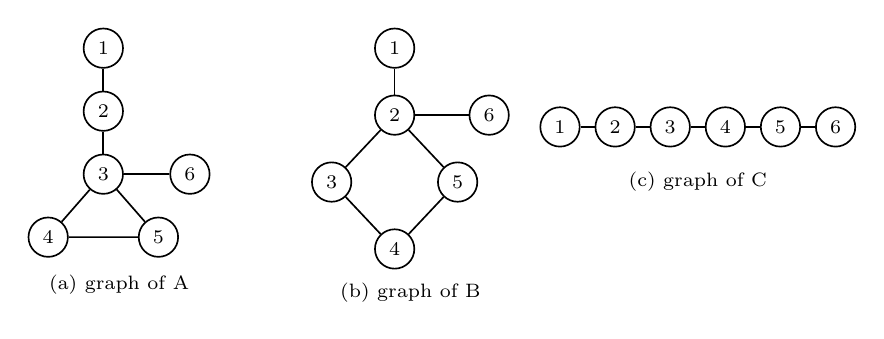
\begin{tikzpicture}[
   vtx/.style={circle,draw,semithick,fill=white,minimum size=5mm,inner sep=0pt,font=\scriptsize},
   every path/.style={semithick}]
  % A: 3-node loop
  \node[vtx](a1) at (0,0){1};   \node[vtx](a2) at (0,-0.8){2};
  \node[vtx](a3) at (0,-1.6){3}; \node[vtx](a6) at (1.1,-1.6){6};
  \node[vtx](a4) at (-0.7,-2.4){4}; \node[vtx](a5) at (0.7,-2.4){5};
  \draw (a1)--(a2)--(a3); \draw (a3)--(a4)--(a5)--(a3); \draw (a3)--(a6);
  \node[font=\scriptsize] at (0.2,-3.0){(a) graph of A};
  % B: 4-node loop (diamond)
  \begin{scope}[xshift=37mm]
    \node[vtx](b1) at (0,0){1};      \node[vtx](b2) at (0,-0.85){2};
    \node[vtx](b6) at (1.2,-0.85){6};
    \node[vtx](b3) at (-0.8,-1.7){3}; \node[vtx](b5) at (0.8,-1.7){5};
    \node[vtx](b4) at (0,-2.55){4};
    \draw (b1)--(b2); \draw (b2)--(b6); \draw (b2)--(b3)--(b4)--(b5)--(b2);
    \node[font=\scriptsize] at (0.2,-3.1){(b) graph of B};
  \end{scope}
  % C: horizontal chain (no loop)
  \begin{scope}[xshift=58mm, yshift=-1.0cm]
    \node[vtx](c1) at (0,0){1};   \node[vtx](c2) at (0.7,0){2};
    \node[vtx](c3) at (1.4,0){3}; \node[vtx](c4) at (2.1,0){4};
    \node[vtx](c5) at (2.8,0){5}; \node[vtx](c6) at (3.5,0){6};
    \draw (c1)--(c2)--(c3)--(c4)--(c5)--(c6);
    \node[font=\scriptsize] at (1.75,-0.7){(c) graph of C};
  \end{scope}
\end{tikzpicture}
\end{minipage}\hfill
\begin{minipage}[c]{0.27\linewidth}
\centering
% grayscale barcode: darkness = lambda / lambda_max, lambda_max = 5.236
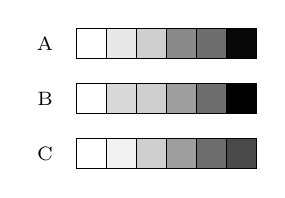
\begin{tikzpicture}[every path/.style={thin}]
  \def\cw{0.38}
  \node[font=\scriptsize] at (-0.4,0)    {A};
  \foreach \i/\p in {0/0,1/9,2/19,3/46,4/57,5/97}
     {\fill[black!\p] (\i*\cw,-0.19) rectangle ++(\cw,0.38);
      \draw (\i*\cw,-0.19) rectangle ++(\cw,0.38);}
  \node[font=\scriptsize] at (-0.4,-0.7) {B};
  \foreach \i/\p in {0/0,1/15,2/19,3/38,4/57,5/100}
     {\fill[black!\p] (\i*\cw,-0.89) rectangle ++(\cw,0.38);
      \draw (\i*\cw,-0.89) rectangle ++(\cw,0.38);}
  \node[font=\scriptsize] at (-0.4,-1.4) {C};
  \foreach \i/\p in {0/0,1/5,2/19,3/38,4/57,5/71}
     {\fill[black!\p] (\i*\cw,-1.59) rectangle ++(\cw,0.38);
      \draw (\i*\cw,-1.59) rectangle ++(\cw,0.38);}
\end{tikzpicture}\\[2pt]
{\scriptsize spectrum as a barcode\\(each cell $=\lambda_i$, darker $=$ larger)}
\end{minipage}

\caption{Three Java fragments, their graphs, and their spectra as a
grayscale barcode. A and B both sum an array and are clones, but A has a
three-node loop and B a four-node loop, so their graphs differ. Their
barcodes still look almost the same, while the unrelated function C, which
has no loop, is lighter in the last cell.}
\label{fig:motivating_exp}
\end{figure*}

Figure~\ref{fig:motivating_exp} shows two Java functions that both sum an
integer array, written with a different loop and different variable names,
together with an unrelated function C that computes a triangle area. As
text, A and B share no identifiers, so token- or line-based comparison
finds little in common between them
\cite{roy2007survey,alomari2020semanticclonebench}. Their graphs are also
not identical: A has a three-node loop and B a four-node loop. Yet if we
take the spectrum (the sorted Laplacian eigenvalues) as the signature of
each graph, A gives $\{0,\,0.485,\,1.000,\,2.425,\,3.000,\,5.089\}$ and B
gives $\{0,\,0.763,\,1.000,\,2.000,\,3.000,\,5.236\}$, which are close, as
the barcodes in the figure show. The unrelated function C gives
$\{0,\,0.268,\,1.000,\,2.000,\,3.000,\,3.732\}$, whose top eigenvalue is
much smaller, so its barcode is visibly lighter. Measuring similarity as the
Euclidean distance between sorted spectra gives $0.53$ for the clone pair
and $1.44$ and $1.58$ for the two non-clone pairs, so a simple threshold
separates them. Because the spectrum is invariant to node relabelling and
changes only a little under small edits to the graph, it matches
behaviourally equivalent code that looks different on the surface. This
motivates our approach and raises its central question: which graph of the
code yields the most informative spectrum for clone detection.

\subsection{Contributions}
\label{subsec:contributions}

The main contributions of this paper are as follows:

\begin{itemize}

    \item \textbf{End-to-End Spectral Representation through Latent Graph Learning}: We propose a learnable spectral code representation in which a fixed-size, weighted latent graph is induced from AST-derived structural information. Its normalized Laplacian spectrum is computed within the learning pipeline and jointly optimized with the latent graph, eliminating the need to manually choose a predefined program graph.

    \item \textbf{Semantic Alignment of Latent Graph Spectra through Clone Supervision}: We use semantic code clone detection to supervise latent graph learning and align the resulting representations with functional equivalence. A Siamese architecture jointly exploits spectral and latent structural information to bring functionally equivalent programs closer while separating non-equivalent ones.

    \item \textbf{Generalization Across Programming Languages}: We systematically evaluate whether the learned representation transfers across programming languages under different training--evaluation configurations, including transfer from well-represented languages to comparatively low-resource target languages without target-language clone supervision. We further investigate whether incorporating cross-language clone pairs during training improves generalization to previously unseen within-language clone detection settings.
\end{itemize}

% For Mohsen to write the first-version

% Proposing a new graph design for source codes that gives us a good spectral representation --> (a) better than AST, CFG, PDG, DDG, etc (traditional graph representations) judged over code clone benchmarks and how good we score. Also, (b) further analysis and backing of the good graph design made by us.

% Empirical study and Exploration of spectral representation over "different graphs of code" on "diverse set of datasets" in "both single-language and cross-language" compared with "Statistical Token based feature space" and "CodeBert Transformer-type embeddings" and "various other CCD approaches that are trained (not baseline but previous work)" using "different metrics" and "eigenvalue + eigenvector" through "other variable and experiments".

% Analytical and a thorough investigation of spectral representation space of source codes and insights and projection operators over that space. --> Eigenvectors and how they can be used for spectral representations in general.

\subsection{Paper Organization}
\label{subsec:outline}

The rest of this paper is organized as follows. \autoref{sec:related_work} reviews related work on code clone
detection, source code representation, and spectral analysis of graphs, and
\autoref{sec:motivating_exp} gives a motivating example. We then present our
graph design and spectral representation, followed by the experimental
setup and the results on single-language and cross-language benchmarks.
Finally, we analyse the spectral representation space and conclude with a
summary and directions for future work.


\section{Related Work}
\label{sec:related_work}

% Our work builds on three lines of research. The first is code clone
% detection. The second is source code representation. The third is
% spectral analysis of graphs. We first review how clone detection has
% moved from text and token matching to learning and graph based semantic
% methods (\autoref{subsec:ccd}). We then describe how source code is
% encoded into the structural and learned representations that detectors
% rely on (\autoref{subsec:representation}). After that we summarise the
% theory and the main applications of graph spectral analysis in other
% fields (\autoref{subsec:spectral}). This last part motivates our use
% of the graph spectrum as a signature of code structure that does not
% depend on node ordering. We close by positioning our contribution against
% this body of work (\autoref{subsec:gap}).

% ---------------------------------------------------------------------
\subsection{Code Clone Detection}
\label{subsec:ccd}

Code clone detection has been studied for more than two decades. Most
techniques are grouped by the program representation on which similarity
is measured. Roy and Cordy \cite{roy2007survey} classify clones into four
types. Type-1 clones are identical except for formatting and naming.
Type-2 and Type-3 clones are syntactically similar but contain small
changes. Type-4 clones implement the same functionality with different
syntax.

\textbf{Text and token based approaches.} The earliest scalable detectors
work on lexical information. \emph{CCFinder} \cite{kamiya2002ccfinder}
normalises token sequences and compares them across several languages.
Ducasse et al.\ \cite{ducasse1999language} detect duplicated code by
matching lines in a language independent way. \emph{CP-Miner}
\cite{li2006cpminer} mines copy-paste bugs in large systems.
\emph{NICAD} \cite{roy2008nicad} adds flexible pretty-printing to line
based comparison so that it can capture near-miss clones. To handle very
large code bases, several token based detectors add indexing and
filtering. \emph{SourcererCC} \cite{sajnani2016sourcerercc} uses an
inverted index. \emph{CCAligner} \cite{wang2018ccaligner} uses
overlapping code windows. \emph{Oreo} \cite{saini2018oreo} uses metric
based filtering. More recently, \emph{StoneDetector}
\cite{heinze2025stonedetector} compares paths taken from dominator trees
of Java source and bytecode. These methods scale well. However, they
mostly ignore code structure, so they have trouble with Type-3 and
Type-4 clones.

\textbf{Tree and graph based approaches.} To capture structural
similarity, detectors began to use the abstract syntax tree (AST).
Baxter et al.\ \cite{baxter1998clone} match subtrees of the AST.
\emph{DECKARD} \cite{jiang2007deckard} describes subtrees with numerical
vectors and clusters them in Euclidean space. Some clones survive
statement reordering or interleaving, which lexical and tree methods miss.
This motivated graph based detectors. Komondoor and Horwitz
\cite{komondoor2001slicing} and Krinke \cite{krinke2001identifying} search
for isomorphic subgraphs of the program dependence graph (PDG). The PDG
uses control flow and data flow rather than surface syntax. Subgraph
isomorphism is expensive to compute, which has limited the scalability of
PDG based methods.

\textbf{Learning and deep learning based approaches.} A large body of
recent work learns similarity directly from data. White et al.\
\cite{white2016deep} were among the first to apply deep learning to clone
detection. They link lexical patterns with syntactic patterns. The
\emph{CDLH} framework \cite{wei2017cdlh} treats functional clone detection
as a supervised hashing problem over AST based LSTMs. \emph{ASTNN}
\cite{zhang2019astnn} splits an AST into statement subtrees and encodes
them with recurrent networks. Tree based convolution
\cite{yu2019neural} and recursive aggregation of ASTs
\cite{buch2019learning} are other structural encoders. Graph neural
networks (GNNs) reduce the semantic gap further. The flow augmented AST
(\emph{FA-AST}) of Wang et al.\ \cite{wang2020faast} adds control flow and
data flow edges to the AST and applies GNNs to measure pairwise
similarity. Graph based semantics learning \cite{yu2023graphsemantics}
combines CFG and PDG representations with attention based graph matching.
\emph{FSD-CLCD} \cite{zhang2024fsdclcd} addresses cross-language detection
through functional semantic distillation over AST derived graphs. Other
work targets efficiency. Transformer based detectors with code token
learners \cite{zhang2023efficient} reduce the cost of attention.
\emph{CCStokener} \cite{wang2023ccstokener} adds semantic information to
tokens. \emph{Code2Img} \cite{hu2023code2img} turns the AST adjacency
matrix into an image and processes it with convolutional networks. The
\emph{BigCloneBench} benchmark \cite{svajlenko2014bigclonebench} is the
standard dataset for evaluating these detectors at scale.

These detectors are accurate, but they have practical costs. GNN and
Transformer based methods need large labelled datasets. They also rely on
costly pairwise comparison and expensive training. In addition, the
learned similarity is often sensitive to node ordering and to graph size.
These limitations motivate representations of code structure that are
compact and do not need heavy training.

% ---------------------------------------------------------------------
\subsection{Source Code Representation}
\label{subsec:representation}

The performance of a clone detector depends heavily on how source code is
represented. The classical representations are explicit program
structures. The AST captures syntax. The control flow graph (CFG) and the
PDG capture execution and dependence relations. The code property graph
(CPG) of Yamaguchi et al.\ \cite{yamaguchi2014cpg} joins syntax, control
flow, and data flow in a single graph, and it has proven effective for
finding vulnerabilities. These graph representations keep rich semantic
information. They are also high dimensional and irregular, which makes
direct comparison difficult.

A second line of work learns continuous representations of code.
\emph{code2vec} \cite{alon2019code2vec} aggregates AST paths into a fixed
length embedding that predicts semantic properties of a snippet.
Pre-trained language models extend this idea to large corpora.
\emph{CodeBERT} \cite{feng2020codebert} learns joint representations of
programming language and natural language. \emph{GraphCodeBERT}
\cite{guo2021graphcodebert} adds data flow structure to the pre-training
objective and improves downstream tasks such as clone detection.
Structure aware neural encoders such as ASTNN \cite{zhang2019astnn} and
FA-AST \cite{wang2020faast} can also be seen as representation learners.
These embeddings are powerful. However, they are learned end to end, they
depend on their training distribution, and they are hard to interpret. In
contrast, our work derives a representation from the algebraic structure
of the code graph itself, so it does not require supervised pre-training.

% ---------------------------------------------------------------------
\subsection{Spectral Analysis of Graphs}
\label{subsec:spectral}

Spectral graph theory studies a graph through the eigenvalues and
eigenvectors of matrices associated with it. The two main matrices are the
adjacency matrix and the graph Laplacian
\cite{chung1997spectral,mohar1991laplacian}. The spectrum encodes global
properties of the graph. Fiedler \cite{fiedler1973algebraic} showed that
the second smallest Laplacian eigenvalue, known as the algebraic
connectivity, measures how well connected a graph is. This result is a
basis for much of modern spectral analysis. The set of eigenvalues does
not change when the vertices are relabelled. This makes the spectrum a
natural signature for comparing graphs of different sizes, which is the
property that AST and PDG comparison needs.

Spectral methods have been successful in many fields. In unsupervised
learning, normalized cuts \cite{shi2000normalized} and the spectral
clustering algorithms of Ng et al.\ \cite{ng2002spectral} and von Luxburg
\cite{vonluxburg2007tutorial} partition data using the leading Laplacian
eigenvectors. In manifold and dimensionality reduction, Laplacian
eigenmaps \cite{belkin2003laplacian} preserve local geometry through the
same eigenbasis. In computer vision and graphics, spectral correspondence
\cite{leordeanu2005spectral} solves matching problems using the principal
eigenvector of an affinity matrix. The heat kernel signature
\cite{sun2009hks} and spectral mesh processing
\cite{zhang2010spectralmesh} use the Laplace--Beltrami spectrum as a shape
descriptor that does not change under isometric deformation. In graph
mining, Weisfeiler--Lehman graph kernels \cite{shervashidze2011wl} compare
graphs through structural features that are refined step by step. Spectral
theory is also the basis of modern graph deep learning. Spectral networks
\cite{bruna2014spectral}, fast localized spectral filtering with Chebyshev
polynomials \cite{defferrard2016cnngraph}, and the graph convolutional
network \cite{kipf2017gcn} all define convolution through the graph
Laplacian spectrum. Later work generalised these ideas with attention
based models \cite{velickovic2018gat}.

The common lesson across these fields is that the graph spectrum gives a
compact description of structure that does not depend on node ordering.
Graph representations of source code are widely used. Even so, the
explicit use of spectral signatures of code graphs for clone detection
has received little attention.

% ---------------------------------------------------------------------
\subsection{Positioning of Our Work}
\label{subsec:gap}

We can summarise the trade-offs as follows. Token and tree based detectors
scale well, but they miss semantic clones. GNN and Transformer based
detectors capture semantics, but they need large labelled corpora and
expensive training, and they are sensitive to graph size and node
ordering. Spectral graph analysis offers the properties that these
detectors lack. It gives a compact descriptor of global graph structure
that does not depend on node ordering and that needs little training. It
also has a long record of success in clustering, shape analysis, and graph
learning. Following this observation, we represent each code fragment as a
graph and describe its structure through the spectrum of its Laplacian.
Clone detection then becomes a comparison of spectral signatures. To the
best of our knowledge, this is the first work to apply spectral analysis
of code graphs to code clone detection in a systematic way. It bridges the
gap between graph models that are rich but heavy and similarity measures
that are light and scalable.


\section{Methodology}
\label{sec:methodology}

SPECTRA-Siam learns the graph underlying a spectral source-code representation
rather than selecting that graph a priori. Given a code fragment, the model
normalizes its language-specific structural information, encodes program
relations, and induces a fixed-size weighted latent graph. A multi-scale
spectral descriptor of this graph is combined with its latent node
representation to obtain the code embedding used for semantic clone detection.


\subsection{Problem Formulation}
\label{sec:problem_formulation}

Let $\mathcal{L}$ denote the set of programming languages considered in this
study, and let $\mathcal{C}_{\ell}$ denote the set of code fragments written
in language $\ell\in\mathcal{L}$. The code space is

\begin{equation}
\label{eq:code_space}
\mathcal{C}
=
\bigcup_{\ell\in\mathcal{L}}
\mathcal{C}_{\ell}.
\end{equation}

For a pair $(c_i,c_j)\in\mathcal{C}\times\mathcal{C}$, let
$y_{ij}\in\{0,1\}$ indicate functional equivalence:

\begin{equation}
\label{eq:clone_label}
y_{ij}
=
\begin{cases}
1, & c_i \equiv_{\mathrm{func}} c_j,\\
0, & \text{otherwise}.
\end{cases}
\end{equation}

Equation~\ref{eq:clone_label} defines equivalence by functionality rather than
lexical or syntactic similarity. Positive pairs may therefore differ in
tokens, program structure, or programming language.

A conventional spectral representation first constructs a predefined program
graph and then extracts its spectrum,

\begin{equation}
\label{eq:fixed_spectral_mapping}
c
\xrightarrow{\mathcal{G}_{b}}
G_b(c)
\xrightarrow{\operatorname{Spec}}
s_b(c),
\end{equation}

where $b$ identifies a graph view such as an Abstract Syntax Tree (AST),
Control Flow Graph (CFG), Data Dependence Graph (DDG), or Code Property Graph
(CPG). Because $\mathcal{G}_{b}$ is fixed independently of the downstream
task, $s_b(c)$ can reflect only the relations represented in $G_b(c)$.

Our formulation makes graph construction part of representation learning.
For code fragment $c$, a parameterized encoder induces

\begin{equation}
\label{eq:learned_graph}
G_{\Theta}(c)
=
\left(
    Z_{\Theta}(c),
    A_{\Theta}(c)
\right),
\end{equation}

where $Z_{\Theta}(c)\in\mathbb{R}^{m\times d}$ contains the latent node states
and $A_{\Theta}(c)\in[0,1]^{m\times m}$ is their learned weighted adjacency.
Its spectral descriptor is

\begin{equation}
\label{eq:learned_spectrum}
s_{\Theta}(c)
=
\operatorname{Spec}_{\Theta}
\left(
    G_{\Theta}(c)
\right).
\end{equation}

The final code representation combines the spectral descriptor with the
latent node states,

\begin{equation}
\label{eq:learned_mapping}
\phi_{\Theta}(c)
=
F_{\Theta}
\left(
    Z_{\Theta}(c),
    s_{\Theta}(c)
\right)
\in
\mathbb{R}^{d_{\phi}}.
\end{equation}

A pairwise prediction head with parameters $\psi$ estimates

\begin{equation}
\label{eq:clone_probability_general}
\hat{y}_{ij}
=
f_{\psi}
\left(
    \phi_{\Theta}(c_i),
    \phi_{\Theta}(c_j)
\right).
\end{equation}

For the labeled pair set

\begin{equation}
\mathcal{D}
=
\left\{
    (c_i,c_j,y_{ij})
\right\},
\end{equation}

training solves

\begin{equation}
\label{eq:central_objective}
(\Theta^{*},\psi^{*})
=
\arg\min_{\Theta,\psi}
\frac{1}{|\mathcal{D}|}
\sum_{(c_i,c_j,y_{ij})\in\mathcal{D}}
\mathcal{L}_{\mathrm{total}}
\left(
    c_i,c_j,y_{ij};
    \Theta,\psi
\right),
\end{equation}

where $\mathcal{L}_{\mathrm{total}}$ is defined in
Equation~\ref{eq:complete_loss}. RQ1 in
Section~\ref{sec:research_questions} examines whether learning
$G_{\Theta}(c)$ under this objective yields a more discriminative spectral
representation than spectral analysis of predefined program graphs.


\subsection{SPECTRA-Siam}
\label{sec:spectra_siam}

Figure~\ref{fig:spectra_overview} summarizes SPECTRA-Siam. Both fragments in
a code pair are processed by the same encoder. Each branch normalizes the
input structure, applies relation-aware encoding, induces a latent graph,
extracts its spectral representation, and combines spectral and latent
features. The resulting code embeddings are passed to a pairwise prediction
head. Sharing encoder parameters places both fragments in the same learned
representation space, following the Siamese learning formulation
\cite{??}.

\begin{figure*}[t]
    \centering
    \safeincludegraphics[width=0.95\textwidth]{figures/main_fig.png}
    \caption{SPECTRA-Siam architecture. A shared encoder maps each code
    fragment to a common representation by normalizing its program structure,
    inducing a weighted latent graph, extracting a multi-scale spectral
    descriptor, and fusing spectral and latent features. The pairwise head
    combines the two code embeddings to estimate semantic clone probability.}
    \label{fig:spectra_overview}
\end{figure*}


\subsubsection{Language-Normalized Structural Encoding}
\label{sec:canonical_structure}

AST node vocabularies are parser- and language-dependent. Equivalent
constructs can consequently receive unrelated raw node labels. We map
parser-specific node types to $K=24$ canonical categories covering control
structures, declarations, expressions, literals, and structural context. For
AST node $v$, $\kappa(t_v)\in\{1,\ldots,K\}$ denotes its canonical category.
Table~\ref{tab:canonical_categories} lists the shared vocabulary.

\begin{table}[t]
\centering
\caption{Canonical AST-node categories shared across the supported programming
languages.}
\label{tab:canonical_categories}
\footnotesize
\renewcommand{\arraystretch}{1.12}
\begin{tabular}{p{0.27\columnwidth}p{0.64\columnwidth}}
\toprule
\textbf{Group} & \textbf{Canonical categories} \\
\midrule
Control &
Control\_If, Control\_Loop, Control\_Switch,
Control\_Return, Control\_Break, Control\_Generic
\\
Declarations &
Var\_Decl, Func\_Decl, Class\_Decl, Param\_Decl
\\
Expressions &
Assign\_Op, Binary\_Op, Unary\_Op,
Call\_Expr, Access\_Expr
\\
Literals &
Literal\_Num, Literal\_Str, Literal\_Bool,
Literal\_Null, Literal\_Generic
\\
Structural / Meta &
Structural\_Block, Identifier\_Context,
Type\_Meta, Canonical\_Unknown
\\
\bottomrule
\end{tabular}
\end{table}

A bounded lexical sketch supplements the canonical node type. Identifiers and
literals are decomposed into subtokens and short character-level features and
mapped deterministically to a fixed set of hash buckets. This mapping is
independent of a vocabulary fitted to the training corpus.

For node $v$, let $\ell_{v1},\ldots,\ell_{vr}$ denote its hashed lexical
features. Its initial representation is

\begin{equation}
\label{eq:node_initial}
h_v^{(0)}
=
\operatorname{LN}
\left(
    E_{\mathrm{can}}
    \left(
        \kappa(t_v)
    \right)
    +
    \gamma_{\mathrm{lex}}
    \frac{1}{r}
    \sum_{q=1}^{r}
    E_{\mathrm{lex}}
    \left(
        \ell_{vq}
    \right)
\right),
\end{equation}

where $E_{\mathrm{can}}$ and $E_{\mathrm{lex}}$ are learned embeddings and

\begin{equation}
\gamma_{\mathrm{lex}}
=
\sigma(g_{\mathrm{lex}})
\end{equation}

controls the lexical contribution. The main configuration does not use raw
source-token embeddings.

The structural encoder operates on AST relations and, when available, DDG
relations projected onto the AST node space. For relation
$r\in\mathcal{R}$, let
$A^{(r)}\in\{0,1\}^{n\times n}$ denote its adjacency matrix. A relation-aware
layer computes

\begin{equation}
\label{eq:relation_encoder}
H^{(l+1)}
=
\operatorname{LN}
\left[
    H^{(l)}
    +
    \operatorname{GELU}
    \left(
        H^{(l)}W_0^{(l)}
        +
        \sum_{r\in\mathcal{R}}
        \widetilde{A}^{(r)}
        H^{(l)}W_r^{(l)}
    \right)
\right],
\end{equation}

where $\widetilde{A}^{(r)}$ is the row-normalized adjacency for relation $r$.
The relation-specific transformations follow established relational
message-passing architectures \cite{??}. The default relation set is

\begin{equation}
\mathcal{R}
=
\{
    \mathrm{AST},
    \mathrm{DDG}
\},
\end{equation}

and the encoder uses two such layers.


\subsubsection{Latent Graph Induction}
\label{sec:latent_graph_induction}

The number of nodes in the encoded program graph varies across fragments.
SPECTRA-Siam maps this representation to $m$ latent nodes,

\begin{equation}
\label{eq:latent_nodes}
Z
=
[z_1,\ldots,z_m]^{\top}
\in
\mathbb{R}^{m\times d},
\end{equation}

where $m=32$. The latent nodes are learned aggregates rather than selected
nodes from the original AST.

Aggregation uses iterative slot attention \cite{??}. For slot query $q_j$ and
encoded-node key $k_v$, the assignment weight is

\begin{equation}
\label{eq:slot_assignment}
P_{vj}
=
\frac{
    \exp
    \left(
        q_j^{\top}k_v/\sqrt{d}
    \right)
}{
    \sum_{u=1}^{m}
    \exp
    \left(
        q_u^{\top}k_v/\sqrt{d}
    \right)
}.
\end{equation}

The main configuration performs three slot updates. The assignment matrix also
maps the latent states back to the encoded-node space,

\begin{equation}
\label{eq:latent_reconstruction}
\widehat{H}
=
PZ,
\end{equation}

giving the reconstruction term

\begin{equation}
\label{eq:reconstruction_loss}
\mathcal{L}_{\mathrm{rec}}
=
\frac{1}{n}
\sum_{v=1}^{n}
\left\|
    h_v-\widehat{h}_v
\right\|_2^2.
\end{equation}

The input topology contributes a separate structural prior. Let
$A_{\mathrm{in}}$ denote the union of the enabled input relations. Its
projection into the latent space is

\begin{equation}
\label{eq:structural_prior}
B
=
\operatorname{Norm}
\left(
    P^{\top}
    A_{\mathrm{in}}
    P
\right),
\end{equation}

where $\operatorname{Norm}(\cdot)$ denotes the normalization applied to the
projected adjacency. The prior $B$ does not determine the final latent
topology.

Latent node affinities are learned independently. For $H_a$ attention heads,

\begin{equation}
\label{eq:latent_score}
S
=
\operatorname{Sym}
\left(
    \frac{1}{H_a}
    \sum_{h=1}^{H_a}
    \frac{
        Q_hK_h^{\top}
    }{
        \sqrt{d_h}
    }
\right)
+
\eta B,
\end{equation}

where

\begin{equation}
\operatorname{Sym}(X)
=
\frac{X+X^{\top}}{2},
\end{equation}

and $\eta$ controls the contribution of the structural prior.

Graph sharpness is conditioned on fragment complexity. We define

\begin{equation}
\chi(c)
=
[
    \nu(c),
    \delta(c)
]^{\top},
\end{equation}

where $\nu(c)$ is normalized node occupancy and $\delta(c)$ is input-edge
density. The corresponding temperature is

\begin{equation}
\label{eq:adaptive_temperature}
T(c)
=
T_{\min}
+
\left(
    T_{\max}-T_{\min}
\right)
\sigma
\left(
    g_T(\chi(c))
\right),
\end{equation}

with $T_{\min}=0.20$ and $T_{\max}=1.20$.

The latent adjacency is

\begin{equation}
\label{eq:latent_adjacency}
A_{\Theta}(c)
=
\operatorname{Sym}
\left[
    \sigma
    \left(
        \frac{S}{T(c)}
    \right)
    \odot
    \left(
        \mathbf{1}\mathbf{1}^{\top}-I_m
    \right)
\right].
\end{equation}

Thus,
$A_{\Theta}(c)\in[0,1]^{m\times m}$ is weighted, symmetric, and has a zero
diagonal. No hard edge-selection threshold is applied. Two graph-refinement
layers update the latent states over $A_{\Theta}(c)$ before spectral
extraction.

The mean off-diagonal edge weight is

\begin{equation}
\label{eq:latent_density}
\rho(A)
=
\frac{1}{m(m-1)}
\sum_{i\neq j}
A_{ij}.
\end{equation}

We regularize this quantity toward $\rho_0=0.15$:

\begin{equation}
\label{eq:density_regularizer}
\mathcal{L}_{\mathrm{graph}}
=
\left(
    \rho(A_{\Theta})-\rho_0
\right)^2.
\end{equation}

The complete transformation from the variable-size encoded program graph to
the learned weighted latent topology is summarized in
Figure~\ref{fig:latent_spectral_core}(a).


\subsubsection{Multi-Scale Spectral Representation}
\label{sec:multiscale_spectral}

The latent adjacency defines the normalized graph Laplacian

\begin{equation}
\label{eq:latent_laplacian}
L_{\Theta}
=
I_m
-
D_{\Theta}^{-1/2}
A_{\Theta}
D_{\Theta}^{-1/2},
\end{equation}

where

\begin{equation}
D_{\Theta}
=
\operatorname{diag}
\left(
    A_{\Theta}\mathbf{1}
\right).
\end{equation}

For a symmetric non-negative adjacency, $L_{\Theta}$ is real symmetric and
its eigenvalues satisfy \cite{??}

\begin{equation}
\label{eq:latent_eigenvalues}
0
\leq
\lambda_1
\leq
\lambda_2
\leq
\cdots
\leq
\lambda_m
\leq
2.
\end{equation}

The spectral descriptor contains three components: eigenvalue density, heat
traces, and Chebyshev spectral energies. Their construction from the learned
latent graph is summarized in
Figure~\ref{fig:latent_spectral_core}(b).

\paragraph{Eigenvalue density.}
For 32 uniformly spaced centers $\xi_j$ on $[0,2]$, we compute

\begin{equation}
\label{eq:eigen_density}
d_j
=
\frac{1}{m}
\sum_{i=1}^{m}
\exp
\left[
    -
    \frac{1}{2}
    \left(
        \frac{
            \lambda_i-\xi_j
        }{
            \sigma_d
        }
    \right)^2
\right],
\end{equation}

with bandwidth $\sigma_d=0.08$.

\paragraph{Heat traces.}
Heat diffusion provides a scale-dependent spectral summary of graph structure
\cite{??}. At diffusion scale $t_q$,

\begin{equation}
\label{eq:heat_trace}
h_q
=
\frac{1}{m}
\sum_{i=1}^{m}
\exp(-t_q\lambda_i).
\end{equation}

The descriptor uses 24 logarithmically spaced scales over

\begin{equation}
t_q
\in
[10^{-2},10^{2}].
\end{equation}

\paragraph{Chebyshev spectral energies.}
The density and heat channels depend on graph topology. To additionally
incorporate signals carried by the latent node states, we learn

\begin{equation}
\label{eq:spectral_signals}
X
=
ZW_s
\in
\mathbb{R}^{m\times R},
\qquad
R=8.
\end{equation}

We use Chebyshev polynomial filtering \cite{??}. Let

\begin{equation}
\widetilde{L}
=
L_{\Theta}-I_m,
\end{equation}

whose spectrum lies in $[-1,1]$. The recurrence is

\begin{align}
\label{eq:cheb_recursion}
T_0(X) &= X, \nonumber\\
T_1(X) &= \widetilde{L}X,\\
T_k(X)
&=
2\widetilde{L}T_{k-1}(X)-T_{k-2}(X),
\qquad k\geq2.
\nonumber
\end{align}

For spectral band $b$,

\begin{equation}
\label{eq:cheb_filter}
Y_b
=
\sum_{k=0}^{K_c}
a_{bk}T_k(X),
\end{equation}

where $K_c=12$. Twelve spectral bands are used.

Band weights depend on the pooled latent state,

\begin{equation}
\label{eq:spectral_attention}
\alpha
=
\operatorname{softmax}
\left(
    W_a\bar{z}
\right),
\qquad
\bar{z}
=
\frac{1}{m}
\sum_{i=1}^{m}z_i.
\end{equation}

The energy for band $b$ and graph signal $r$ is

\begin{equation}
\label{eq:spectral_energy}
e_{br}
=
\alpha_b
\frac{1}{m}
\sum_{i=1}^{m}
Y_b(i,r)^2.
\end{equation}

The eigenvalue-density and heat-trace channels use the eigenspectrum as
descriptor input. Gradients are not propagated through their ordered
eigenvalues. In contrast, the Chebyshev branch acts directly on
$L_{\Theta}$ and therefore supplies the differentiable spectral path to the
learned adjacency.

The complete spectral descriptor is

\begin{equation}
\label{eq:complete_spectral_descriptor}
s_{\Theta}(c)
=
\left[
    d(c)
    \,\Vert\,
    h(c)
    \,\Vert\,
    e(c)
\right]
\in
\mathbb{R}^{152},
\end{equation}

with 32 density features, 24 heat-trace features, and 96 Chebyshev-energy
features.

\begin{figure*}[t]
    \centering
    \begin{minipage}[t]{0.49\textwidth}
        \centering
        \safeincludegraphics[width=\linewidth]{figures/latent_graph_induction.png}
    \end{minipage}
    \hfill
    \begin{minipage}[t]{0.49\textwidth}
        \centering
        \safeincludegraphics[width=\linewidth]{figures/multiscale_spectral_representation.png}
    \end{minipage}
    \caption{Latent graph induction and spectral representation.
    \textbf{(a)} Soft slot assignments map the variable-size encoded program
    graph to a fixed set of latent nodes. Learned latent affinities, the
    projected structural prior, and the adaptive temperature jointly determine
    the weighted adjacency $A_{\Theta}$; reconstruction and graph-density
    terms constrain the induced representation.
    \textbf{(b)} The normalized Laplacian of $A_{\Theta}$ is represented
    through eigenvalue density, heat traces, and Chebyshev spectral energies.
    The three channels contribute 32, 24, and 96 features, respectively,
    forming the 152-dimensional descriptor $s_{\Theta}(c)$.}
    \label{fig:latent_spectral_core}
\end{figure*}


\subsubsection{Spectral--Latent Fusion and Pairwise Prediction}
\label{sec:spectral_latent_fusion}

The latent states are pooled as

\begin{equation}
\label{eq:latent_mean}
\bar{z}(c)
=
\frac{1}{m}
\sum_{i=1}^{m}
z_i(c).
\end{equation}

Let $g_{\Theta}$ denote the spectral projection and
$f_{\mathrm{out}}$ the fusion network. The code embedding is

\begin{equation}
\label{eq:code_embedding}
\phi_{\Theta}(c)
=
\operatorname{Norm}_2
\left[
    f_{\mathrm{out}}
    \left(
        \bar{z}(c)
        \,\Vert\,
        g_{\Theta}
        \left(
            s_{\Theta}(c)
        \right)
    \right)
\right].
\end{equation}

For pair $(c_i,c_j)$, write

\begin{equation}
\phi_i
=
\phi_{\Theta}(c_i),
\qquad
\phi_j
=
\phi_{\Theta}(c_j).
\end{equation}

The pairwise feature vector is

\begin{equation}
\label{eq:pair_representation}
q_{ij}
=
\left[
    \phi_i
    \,\Vert\,
    \phi_j
    \,\Vert\,
    |\phi_i-\phi_j|
    \,\Vert\,
    \phi_i\odot\phi_j
    \,\Vert\,
    \cos(\phi_i,\phi_j)
\right].
\end{equation}

A two-layer prediction network maps $q_{ij}$ to logit $a_{ij}$ and clone
probability

\begin{equation}
\label{eq:pair_probability}
p_{ij}
=
\sigma(a_{ij}).
\end{equation}


\subsubsection{Training Objective}
\label{sec:training_objective}

The primary objective is class-weighted binary cross entropy,

\begin{equation}
\label{eq:classification_loss}
\mathcal{L}_{\mathrm{cls}}
=
-
\frac{1}{|\mathcal{B}|}
\sum_{(i,j)\in\mathcal{B}}
\left[
    w_{+}y_{ij}\log p_{ij}
    +
    (1-y_{ij})\log(1-p_{ij})
\right],
\end{equation}

where $w_{+}$ is determined from the training-set class distribution.

Spectral descriptors receive an additional contrastive objective. Let

\begin{equation}
\label{eq:spectral_cosine}
c_{ij}^{s}
=
\cos
\left(
    s_{\Theta}(c_i),
    s_{\Theta}(c_j)
\right).
\end{equation}

The spectral contrastive term is

\begin{equation}
\label{eq:spectral_loss}
\mathcal{L}_{\mathrm{spec}}
=
\frac{1}{|\mathcal{B}|}
\sum_{(i,j)\in\mathcal{B}}
\left[
    y_{ij}(1-c_{ij}^{s})^2
    +
    (1-y_{ij})
    \left[
        c_{ij}^{s}-\mu_s
    \right]_{+}^{2}
\right],
\end{equation}

where $\mu_s=0.25$.

Hard negatives are selected in the fused embedding space. With

\begin{equation}
c_{ij}^{\phi}
=
\cos(\phi_i,\phi_j),
\end{equation}

let $\mathcal{H}^{-}$ contain non-clone pairs satisfying
$c_{ij}^{\phi}>\mu_h$, restricted to the highest-scoring 25\% within a batch.
The corresponding term is

\begin{equation}
\label{eq:hard_negative_loss}
\mathcal{L}_{\mathrm{hard}}
=
\frac{1}{|\mathcal{H}^{-}|}
\sum_{(i,j)\in\mathcal{H}^{-}}
\left[
    c_{ij}^{\phi}-\mu_h
\right]_{+}^{2},
\end{equation}

with $\mu_h=0.10$.

The complete objective is

\begin{equation}
\label{eq:complete_loss}
\boxed{
\mathcal{L}_{\mathrm{total}}
=
\mathcal{L}_{\mathrm{cls}}
+
0.30\,\mathcal{L}_{\mathrm{spec}}
+
0.20\,\mathcal{L}_{\mathrm{hard}}
+
0.05\,\mathcal{L}_{\mathrm{rec}}
+
0.01\,\mathcal{L}_{\mathrm{graph}}
}.
\end{equation}


\subsubsection{Optimization}
\label{sec:training_procedure}

Training uses AdamW \cite{??}. The eigensolver associated with the
eigenvalue-density and heat-trace channels is evaluated without propagating
gradients through the ordered eigenvalues. The Chebyshev branch in
Equations~\ref{eq:cheb_recursion}--\ref{eq:spectral_energy} operates directly
on $L_{\Theta}$ and supplies the spectral gradient path to
$A_{\Theta}$. The remaining architecture and optimization settings are
reported in Section~\ref{sec:exp_settings}.


\section{Experimental Design}
\label{sec:exp_design}

The experiments examine the contribution of latent graph learning to spectral
clone detection, compare SPECTRA-Siam with existing clone-detection methods,
and evaluate generalization across programming languages.


\subsection{Research Questions}
\label{sec:research_questions}

\begin{itemize}
    \item \textbf{RQ1.} \textit{To what extent does latent graph learning
    improve the performance of spectral code clone detection over conventional
    program-graph spectral baselines?}

    \vspace{1em}

    \item \textbf{RQ2.} \textit{How does the proposed spectral latent-graph
    approach compare with existing code clone detection methods?}

    \vspace{1em}

    \item \textbf{RQ3.} \textit{How well does the proposed approach generalize
    across programming languages under different within- and cross-language
    training settings?}
\end{itemize}


\subsection{Datasets and Split Integrity}
\label{subsec:datasets}

The experiments use four prepared V3 benchmark bundles. The counts in
Table~\ref{tab:datasets} are read from the metadata consumed by the graph
pipeline; they are therefore the counts of the actual experimental splits,
not headline totals from a different release of a benchmark. In each split,
``all / clone'' gives the number of labelled pairs and the number of positive
clone pairs; the number of non-clone pairs is their difference.

\begin{table*}[t]
\centering
\caption{Prepared benchmark composition before graph-coverage filtering. Pair
counts preserve the supplied train/validation/test partitions.}
\label{tab:datasets}
\small
\renewcommand{\arraystretch}{1.12}
\begin{tabular}{lllrrr}
\toprule
Dataset & Languages & Fragments & \shortstack{Train pairs\\all / clone} &
\shortstack{Validation pairs\\all / clone} & \shortstack{Test pairs\\all / clone} \\
\midrule
BigCloneBench (CodeXGLUE) & Java & $9{,}126$ & $901{,}028 / 450{,}862$ & $415{,}416 / 53{,}839$ & $415{,}416 / 56{,}820$ \\
AtCoder & Java, Python & $43{,}143$ & $544{,}054 / 272{,}027$ & $116{,}704 / 58{,}352$ & $116{,}736 / 58{,}368$ \\
GPTCloneBench & C, C\#, Java, Python & $5{,}924$ & $12{,}432 / 6{,}216$ & $2{,}658 / 1{,}329$ & $2{,}682 / 1{,}341$ \\
SemanticCloneBench & C, C\#, Java, Python & $8{,}000$ & $5{,}836 / 2{,}918$ & $1{,}084 / 542$ & $1{,}080 / 540$ \\
\bottomrule
\end{tabular}
\end{table*}

\paragraph{BigCloneBench (CodeXGLUE).}
The Java benchmark uses the stored official CodeXGLUE split without resampling
or relabelling. The final \method{} run retains
$900{,}850/415{,}416/415{,}416$ graph-evaluable train/validation/test pairs.

\paragraph{AtCoder.}
The prepared problem-disjoint split contains accepted Java and Python
solutions. Positive Java--Python pairs solve the same problem, and negative
pairs solve different problems. The final \method{} run retains
$544{,}054/116{,}704/116{,}736$ graph-evaluable pairs.

\paragraph{GPTCloneBench.}
The multilingual prepared split is author-group safe. It contains
$17{,}772$ labelled pairs over $5{,}924$ unique endpoints and is class
balanced in each partition. The final \method{} run retains
$12{,}335/2{,}619/2{,}663$ graph-evaluable pairs.

\paragraph{SemanticCloneBench.}
The semantic-group-disjoint benchmark contains $2{,}000$ fragments in each
of C, C\#, Java, and Python. Its $8{,}000$ labelled pairs are class balanced
within each supplied partition. The final \method{} run retains
$5{,}825/1{,}082/1{,}078$ graph-evaluable pairs.

Pairs are retained for a method only when both endpoints have every required
representation. Each result artifact records the resulting split sizes. When
coverage differs between methods, a strict pairwise claim requires their common
evaluable pair IDs or an explicit disclosure of the differing sample sizes.

\subsection{Baselines}
\label{sec:baselines}

The evaluation includes pretrained code models, graph- and tree-based clone
detectors, and fixed graph-spectral representations. The fixed spectral
baselines provide the direct comparison for RQ1; the remaining methods place
SPECTRA-Siam within the broader clone-detection literature.


\subsubsection{Transformer-based Pretrained Models}
\label{sec:pretrained_baselines}

The pretrained comparison includes CodeBERT \cite{??},
GraphCodeBERT \cite{??}, CodeT5 \cite{??}, and UniXCoder \cite{??}.
Each encoder produces a fixed-dimensional representation for a code fragment.
These baselines were implemented by a collaborator and are reported separately
from the methods executed by this repository.

Three downstream configurations are considered. \emph{No Train} compares
embeddings directly using cosine similarity and fits no task-specific
classifier. Random Forest (RF) and a Siamese Neural Network (SNN) provide
supervised alternatives. All continuous-score configurations use the
validation-based threshold-selection procedure in
Section~\ref{sec:evaluation_settings}.

For the dimensionality-controlled variants, PCA reduces each pretrained
representation to 32 components. The PCA transformation is fitted on
training-fragment embeddings only and is subsequently applied unchanged to
validation and test embeddings.


\subsubsection{Graph- and Tree-based Learning Approaches}
\label{sec:graph-based_baselines}

Graph Neural Network (GNN) encoders are evaluated independently on AST, CFG,
DDG, and CPG representations. If a required graph cannot be constructed for a
fragment, that representation is treated as unavailable rather than replaced
by an empty graph.

The additional clone-detection baselines are DECKARD \cite{??},
RtvNN \cite{??}, CDLH \cite{??}, DeepSim \cite{??}, ASTNN \cite{??},
FA-AST+GGNN \cite{??}, and FA-AST+GMN \cite{??}. Retrained baselines use the
same prepared partitions as SPECTRA-Siam. Published scores obtained under
different split or negative-sampling protocols are not mixed with the
controlled results.


\subsubsection{Graph Spectral Baselines}
\label{sec:spectral_baselines}

RQ1 compares SPECTRA-Siam with spectra derived from predefined program graphs.
The candidate graph representations are AST, CFG, Program Dependence Graph
(PDG), DDG, and CPG. The graph export used in the experiments contains
independent AST, CFG, DDG, and CPG views. PDG is therefore evaluated only
where an independent PDG representation is available; an unavailable PDG is
not replaced by another graph representation or interpreted as an empty
graph.

For graph type $b$, let $\lambda(G_b(c))$ denote its ordered spectrum. The
fixed spectral representation is

\begin{equation}
\label{eq:fixed_spectral_vector}
x_b(c)
=
\left[
    \operatorname{Stat}
    \left(
        \lambda(G_b(c))
    \right)
    \,\Vert\,
    \lambda_{1:64}(G_b(c))
\right],
\end{equation}

where $\operatorname{Stat}(\cdot)$ contains spectral length, mean, standard
deviation, minimum, maximum, and the 25th, 50th, and 75th percentiles.
Spectra longer than 64 values are truncated, whereas shorter spectra are
zero-padded.

\paragraph{No Train.}
Without a task-specific classifier, pair similarity is

\begin{equation}
\label{eq:no_train_spectral_similarity}
s_b(c_i,c_j)
=
\frac{
    1
}{
    1+
    \left\|
        x_b(c_i)-x_b(c_j)
    \right\|_2
}.
\end{equation}

\emph{No Train} refers to the absence of classifier training; the decision
threshold is still selected using validation data.

\paragraph{Logistic Regression and Random Forest.}
Both classifiers receive the pairwise representation

\begin{equation}
\label{eq:spectral_pair_features}
r_{ij}
=
\left[
    |x_i-x_j|
    \,\Vert\,
    x_i\odot x_j
    \,\Vert\,
    \cos(x_i,x_j)
    \,\Vert\,
    \|x_i-x_j\|_2
\right].
\end{equation}

The Random Forest contains 200 trees, has maximum depth 16, and uses a minimum
leaf size of 5.

\paragraph{Spectral Siamese Neural Network.}
The final fixed-spectral baseline trains an SNN over the predefined graph
spectrum. Both this model and SPECTRA-Siam receive pairwise semantic clone
supervision; only SPECTRA-Siam learns the graph on which its spectral
representation is defined. This comparison therefore controls for the effect
of Siamese supervision while isolating the contribution of latent graph
learning.


\subsection{Experimental Setting}
\label{sec:exp_settings}

The same train, validation, and test partitions are maintained throughout the
study. Training data determine model parameters, validation data determine
checkpoints and classification thresholds, and test data are reserved for
final evaluation.

A pair is evaluated by a method only when all representations required by
that method can be constructed. Each run records the resulting numbers of
training, validation, and test pairs. When representation coverage differs
between two methods, direct comparisons are additionally computed over their
common evaluable pair IDs so that differences in representation coverage are
not conflated with predictive performance.

The primary experiments use all representation-evaluable pairs. Controlled
development experiments use at most
$50{,}000/10{,}000/10{,}000$
training/validation/test pairs when the corresponding dataset is sufficiently
large. All stochastic components use random seed 42.

SPECTRA-Siam is trained for four epochs with AdamW, using a learning rate of
$10^{-4}$ and weight decay of $10^{-4}$. The physical batch size is 32, and
gradient accumulation yields an effective batch size of 128. GPU training
uses mixed precision, while numerically sensitive spectral operations remain
in single precision \cite{??}. Table~\ref{tab:experimental_settings}
summarizes the main configuration.

\begin{table}[t]
\centering
\caption{SPECTRA-Siam configuration used in the main experiments.}
\label{tab:experimental_settings}
\footnotesize
\renewcommand{\arraystretch}{1.12}
\begin{tabular}{ll}
\toprule
\textbf{Parameter} & \textbf{Value} \\
\midrule
Maximum AST nodes & 256 \\
Canonical node categories & 24 \\
Hidden dimension & 256 \\
Latent nodes & 32 \\
Slot-attention iterations & 3 \\
Latent attention heads & 4 \\
Structural relations & AST + DDG \\
Target latent-graph density & 0.15 \\
Temperature range & $[0.20,1.20]$ \\
\midrule
Eigenvalue-density bins & 32 \\
Density bandwidth & 0.08 \\
Heat-trace scales & 24 \\
Heat-scale interval & $[10^{-2},10^{2}]$ \\
Spectral bands & 12 \\
Learned graph signals & 8 \\
Chebyshev degree & 12 \\
Spectral descriptor size & 152 \\
\midrule
Optimizer & AdamW \\
Learning rate & $10^{-4}$ \\
Weight decay & $10^{-4}$ \\
Physical batch size & 32 \\
Effective batch size & 128 \\
Training epochs & 4 \\
Spectral-loss weight & 0.30 \\
Hard-negative weight & 0.20 \\
Reconstruction-loss weight & 0.05 \\
Graph-regularization weight & 0.01 \\
Hard-negative fraction & 0.25 \\
Random seed & 42 \\
\bottomrule
\end{tabular}
\end{table}

Learned models are executed on an NVIDIA T4 GPU where applicable. The
No-Train, Logistic Regression, and Random Forest spectral baselines operate
on precomputed representations and run on CPU. Trainable parameter count and
end-to-end runtime are recorded for the final experiments. Runtime comparisons
are restricted to runs performed under comparable hardware and data coverage.


\subsection{Evaluation Protocol}
\label{sec:evaluation_settings}

For every method producing a continuous clone score, the classification
threshold is selected exclusively on validation data. Let $\mathcal{T}$ denote
the candidate thresholds. We first identify

\begin{equation}
\label{eq:f1_optimal_thresholds}
\mathcal{T}_{F1}
=
\arg\max_{\tau\in\mathcal{T}}
F1_{\mathrm{val}}(\tau),
\end{equation}

and use balanced accuracy to resolve ties:

\begin{equation}
\label{eq:validation_threshold}
\tau^{*}
=
\arg\max_{\tau\in\mathcal{T}_{F1}}
BA_{\mathrm{val}}(\tau).
\end{equation}

The selected threshold $\tau^{*}$ is fixed before test evaluation.


\subsubsection{RQ1: Learned vs. Conventional Spectral Representations}
\label{sec:rq1_evaluation}

RQ1 compares SPECTRA-Siam with the fixed graph-spectral baselines in
Section~\ref{sec:spectral_baselines}. The No-Train configuration evaluates
the predefined spectrum without a learned classifier. Logistic Regression and
Random Forest introduce conventional supervised decision functions, while
the spectral SNN adds pairwise neural supervision without changing the
underlying program graph.

The fixed spectral SNN provides the most direct control for latent graph
learning. Both models receive pairwise semantic clone supervision, but only
SPECTRA-Siam optimizes the topology from which its spectral representation is
derived.


\subsubsection{RQ2: Comparison with Clone Detection Methods}
\label{sec:rq2_evaluation}

RQ2 compares SPECTRA-Siam with the pretrained, graph-based, and tree-based
methods described in Section~\ref{sec:baselines}. All methods follow the same
benchmark partitioning protocol. The primary comparison reports Precision,
Recall, F1, and Accuracy. Macro-F1 and Balanced Accuracy are additionally
reported for imbalanced subsets. Parameter count and runtime are reported
separately from predictive performance.


\subsubsection{RQ3: Generalization Across Programming Languages}
\label{sec:rq3_evaluation}

RQ3 distinguishes cross-language clone detection from generalization across
programming languages. A Java--C pair is a cross-language clone instance
because its endpoints use different programming languages. By contrast,
training on Java--Java pairs and evaluating on C--C pairs measures transfer
across languages while keeping the test task within-language.

Let $\mathcal{D}_{a,b}^{r}$ denote pairs whose endpoints use languages $a$
and $b$, where

\begin{equation}
r
\in
\{
    \mathrm{tr},
    \mathrm{va},
    \mathrm{te}
\}
\end{equation}

denotes the training, validation, or test partition. The two generalization
protocols are summarized in Figure~\ref{fig:language_transfer_protocol}:
panel~(a) shows monolingual-source transfer and panel~(b) shows
cross-language bridge supervision.

\paragraph{Monolingual-source transfer.}
The first regime trains only on within-language source pairs,

\begin{equation}
\label{eq:within_language_transfer}
(\Theta^{*},\psi^{*})
=
\operatorname{Train}
\left(
    \mathcal{D}_{s,s}^{\mathrm{tr}}
\right),
\qquad
\tau^{*}
=
\operatorname{Select}
\left(
    \mathcal{D}_{s,s}^{\mathrm{va}}
\right).
\end{equation}

For target language $t\neq s$, the frozen model and validation-selected
threshold are evaluated on

\begin{equation}
\label{eq:target_language_evaluation}
\operatorname{Eval}
\left(
    \Theta^{*},
    \psi^{*},
    \tau^{*};
    \mathcal{D}_{t,t}^{\mathrm{te}}
\right).
\end{equation}

A representative transfer is

\begin{equation}
\label{eq:java_to_c}
\mathrm{Java}\!-\!\mathrm{Java}
\longrightarrow
\mathrm{C}\!-\!\mathrm{C}.
\end{equation}

In this example, no C--C pair contributes to either training or validation,
as illustrated in Figure~\ref{fig:language_transfer_protocol}(a).

\paragraph{Cross-language bridge supervision.}
The second regime augments source-language supervision with source--target
cross-language pairs:

\begin{align}
\label{eq:bridge_supervision}
\mathcal{D}_{\mathrm{bridge}}^{\mathrm{tr}}
&=
\mathcal{D}_{s,s}^{\mathrm{tr}}
\cup
\mathcal{D}_{s,t}^{\mathrm{tr}},
\\
\mathcal{D}_{\mathrm{bridge}}^{\mathrm{va}}
&=
\mathcal{D}_{s,s}^{\mathrm{va}}
\cup
\mathcal{D}_{s,t}^{\mathrm{va}}.
\end{align}

Training and threshold selection use these partitions,

\begin{equation}
(\Theta^{*},\psi^{*})
=
\operatorname{Train}
\left(
    \mathcal{D}_{\mathrm{bridge}}^{\mathrm{tr}}
\right),
\qquad
\tau^{*}
=
\operatorname{Select}
\left(
    \mathcal{D}_{\mathrm{bridge}}^{\mathrm{va}}
\right),
\end{equation}

while evaluation remains on $\mathcal{D}_{t,t}^{\mathrm{te}}$. For example,

\begin{equation}
\label{eq:bridge_example}
\left(
    \mathrm{Java}\!-\!\mathrm{Java}
    +
    \mathrm{Java}\!-\!\mathrm{C}
\right)
\longrightarrow
\mathrm{C}\!-\!\mathrm{C}.
\end{equation}

Here, Java--C pairs provide cross-language bridge supervision, whereas C--C
pairs remain absent from both training and validation, as shown in
Figure~\ref{fig:language_transfer_protocol}(b). Comparing
Equations~\ref{eq:java_to_c} and~\ref{eq:bridge_example} measures the effect
of bridge supervision on subsequent within-language target performance.

Target-test pairs are used only for final scoring. Model parameters,
checkpoints, thresholds, and other data-dependent transformations are fixed
before target-test evaluation. Results are organized as
source-language $\times$ target-language matrices over Java, Python, C, and
C\#. Diagonal cells correspond to conventional within-language training and
evaluation, whereas off-diagonal cells represent generalization to a different
programming language. Bridge-supervision results are reported where the
required source--target pairs are available.

Each transfer configuration uses only structural relations supported
consistently by the languages involved.

\begin{figure}[t]
    \centering
    \begin{minipage}[t]{\linewidth}
        \centering
        \safeincludegraphics[width=\linewidth]{figures/monolingual_source_transfer.png}
    \end{minipage}

    \vspace{0.4em}

    \begin{minipage}[t]{\linewidth}
        \centering
        \safeincludegraphics[width=\linewidth]{figures/cross_language_bridge_alignment.png}
    \end{minipage}

    \caption{Generalization protocols used for RQ3.
    \textbf{(a)} Monolingual-source transfer uses only source-language
    within-language pairs for training and validation before evaluation on
    within-language pairs from a different target language.
    \textbf{(b)} Cross-language bridge supervision additionally introduces
    source--target pairs during training and validation, while target--target
    pairs remain withheld until final evaluation.}
    \label{fig:language_transfer_protocol}
\end{figure}


\subsubsection{Metrics}
\label{sec:metrics}

Let $TP$, $FP$, $TN$, and $FN$ denote the confusion-matrix counts with clone
as the positive class. Precision, Recall, F1, and Accuracy are

\begin{align}
\label{eq:precision_metric}
\mathrm{Precision}
&=
\frac{TP}{TP+FP},
\\
\label{eq:recall_metric}
\mathrm{Recall}
&=
\frac{TP}{TP+FN},
\\
\label{eq:f1_metric}
F1
&=
2
\frac{
    \mathrm{Precision}\cdot\mathrm{Recall}
}{
    \mathrm{Precision}+\mathrm{Recall}
},
\\
\label{eq:accuracy_metric}
\mathrm{Accuracy}
&=
\frac{
    TP+TN
}{
    TP+TN+FP+FN
}.
\end{align}

F1 is the primary metric. For imbalanced subsets, we additionally report

\begin{equation}
\label{eq:macro_f1_metric}
\mathrm{MacroF1}
=
\frac{
    F1_{\mathrm{clone}}
    +
    F1_{\mathrm{nonclone}}
}{2},
\end{equation}

and

\begin{equation}
\label{eq:balanced_accuracy_metric}
BA
=
\frac{1}{2}
\left(
    \frac{TP}{TP+FN}
    +
    \frac{TN}{TN+FP}
\right).
\end{equation}

For RQ3, these metrics are reported separately for each source--target
language configuration rather than only as an aggregate multilingual score.

\section{Experimental Results}
\label{sec:exp_results}

The result tables distinguish two provenance classes. Controlled repository
runs are read from \texttt{wide\_test\_metrics.csv}; independently implemented
pretrained baselines are transcribed from the collaborator benchmark report and
archived in \texttt{pretrained\_collaborator\_results.csv}. BigCloneBench in
the tables denotes the stored CodeXGLUE binary-clone split. Separating the two
sources preserves the pretrained results without implying that their missing
runtime and training metadata were reproduced by this repository.

\subsection{RQ1: Controlled Repository Results}
\label{sec:rq}

Table~\ref{tab:results_baselines_overall} reports the test metrics available in
the final repository artifact. The fixed-spectrum rows directly test whether a
learned latent graph improves over spectra of predefined AST, CFG, DDG, and CPG
views; the remaining rows provide controlled code-representation baselines.

\begin{table*}[t]
\centering
\caption{Test performance of methods executed by the repository pipeline. All values are read from the archived final benchmark artifact; P, R, and Acc denote precision, recall, and accuracy.}
\label{tab:results_baselines_overall}
\scriptsize
\setlength{\tabcolsep}{2.2pt}
\renewcommand{\arraystretch}{1.08}
\resizebox{\textwidth}{!}{%
\begin{tabular}{l*{16}{c}}
\toprule
Method & \multicolumn{4}{c}{\shortstack{BigCloneBench\\(CodeXGLUE)}} & \multicolumn{4}{c}{SemanticCloneBench} & \multicolumn{4}{c}{GPTCloneBench} & \multicolumn{4}{c}{ATCoder} \\
\cmidrule(lr){2-5}\cmidrule(lr){6-9}\cmidrule(lr){10-13}\cmidrule(lr){14-17}
 & P & R & F1 & Acc & P & R & F1 & Acc & P & R & F1 & Acc & P & R & F1 & Acc \\
\midrule
\multicolumn{17}{l}{\textit{Observed-graph GNN baselines}} \\
GNN-AST & 0.2593 & 0.4192 & 0.3204 & 0.7568 & 0.5283 & 0.8981 & 0.6653 & 0.5481 & 0.9284 & 0.8128 & 0.8668 & 0.8751 & 0.5000 & 1.0000 & 0.6667 & 0.5000 \\
GNN-CFG & 0.2621 & 0.3482 & 0.2991 & 0.7767 & 0.5000 & 1.0000 & 0.6667 & 0.5000 & 0.6515 & 0.9090 & 0.7590 & 0.7114 & 0.5000 & 1.0000 & 0.6667 & 0.5000 \\
GNN-DDG & 0.2446 & 0.5007 & 0.3286 & 0.7202 & 0.5182 & 0.9741 & 0.6765 & 0.5343 & 0.8411 & 0.8054 & 0.8229 & 0.8266 & 0.5000 & 0.9997 & 0.6666 & 0.5000 \\
GNN-CPG & 0.3375 & 0.4328 & 0.3793 & 0.8062 & 0.4981 & 0.9574 & 0.6553 & 0.4963 & 0.9173 & 0.8024 & 0.8560 & 0.8650 & 0.5000 & 1.0000 & 0.6667 & 0.5000 \\
\addlinespace[2pt]
\multicolumn{17}{l}{\textit{Token/tree code baselines}} \\
Deckard & 0.1536 & 0.8416 & 0.2597 & 0.3439 & 0.6238 & 0.8444 & 0.7175 & 0.6676 & 0.9612 & 0.9045 & 0.9320 & 0.9340 & 0.5000 & 1.0000 & 0.6667 & 0.5000 \\
RtvNN & 0.9348 & 0.8989 & 0.9165 & 0.9776 & 0.7332 & 0.8500 & 0.7873 & 0.7704 & 0.9628 & 0.9068 & 0.9339 & 0.9359 & 0.8646 & 0.9151 & 0.8891 & 0.8859 \\
CDLH & 0.9420 & 0.9404 & 0.9412 & 0.9839 & 0.6643 & 0.8722 & 0.7542 & 0.7157 & 0.9618 & 0.9210 & 0.9410 & 0.9422 & 0.8597 & 0.8992 & 0.8790 & 0.8762 \\
\addlinespace[2pt]
\multicolumn{17}{l}{\textit{Other graph-based learning methods}} \\
ASTNN & 0.6455 & 0.7052 & 0.6740 & 0.9065 & 0.5690 & 0.9167 & 0.7021 & 0.6111 & 0.7789 & 0.8551 & 0.8152 & 0.8061 & 0.5000 & 0.9990 & 0.6664 & 0.4999 \\
DeepSim & 0.9073 & 0.8606 & 0.8833 & 0.9689 & 0.6381 & 0.8426 & 0.7263 & 0.6824 & 0.9430 & 0.9001 & 0.9210 & 0.9228 & 0.7572 & 0.8741 & 0.8114 & 0.7969 \\
FA-AST+GGNN & 0.6565 & 0.5502 & 0.5987 & 0.8991 & 0.5445 & 0.8389 & 0.6603 & 0.5685 & 0.9506 & 0.8173 & 0.8789 & 0.8874 & 0.5000 & 1.0000 & 0.6667 & 0.5000 \\
FA-AST+GMN & 0.6238 & 0.6422 & 0.6328 & 0.8981 & 0.5234 & 0.9130 & 0.6653 & 0.5407 & 0.9062 & 0.8285 & 0.8656 & 0.8714 & 0.5000 & 1.0000 & 0.6667 & 0.5000 \\
\addlinespace[2pt]
\multicolumn{17}{l}{\textit{Proposed method}} \\
\textbf{SPECTRA-Siam} & 0.7195 & 0.7018 & 0.7105 & 0.9216 & 0.6514 & 0.7648 & 0.7036 & 0.6778 & 0.9459 & 0.8491 & 0.8949 & 0.9003 & 0.7709 & 0.9032 & 0.8318 & 0.8174 \\
\addlinespace[2pt]
\multicolumn{17}{l}{\textit{Fixed spectral-representation baselines}} \\
AST + No Train & 0.1461 & 0.7940 & 0.2468 & 0.3355 & 0.5014 & 0.9963 & 0.6671 & 0.5028 & 0.9226 & 0.7924 & 0.8526 & 0.8629 & 0.5000 & 1.0000 & 0.6667 & 0.5000 \\
AST + RF & 0.3297 & 0.4364 & 0.3756 & 0.8011 & 0.5399 & 0.8778 & 0.6685 & 0.5648 & 0.9149 & 0.8506 & 0.8816 & 0.8857 & 0.5000 & 0.9999 & 0.6667 & 0.5000 \\
AST + LR & 0.1778 & 0.5599 & 0.2699 & 0.5848 & 0.5756 & 0.7685 & 0.6582 & 0.6009 & 0.9062 & 0.8514 & 0.8779 & 0.8816 & 0.5000 & 1.0000 & 0.6667 & 0.5000 \\
AST + SNN & 0.4232 & 0.4138 & 0.4185 & 0.8427 & 0.5234 & 0.9130 & 0.6653 & 0.5407 & 0.9266 & 0.8285 & 0.8748 & 0.8814 & 0.5000 & 1.0000 & 0.6667 & 0.5000 \\
CFG + No Train & 0.1372 & 0.9998 & 0.2413 & 0.1381 & 0.5000 & 0.9974 & 0.6661 & 0.5000 & 0.9396 & 0.7356 & 0.8252 & 0.8441 & 0.5003 & 1.0000 & 0.6669 & 0.5003 \\
CFG + RF & 0.2439 & 0.4792 & 0.3233 & 0.7250 & 0.5489 & 0.9205 & 0.6877 & 0.5821 & 0.8500 & 0.8618 & 0.8558 & 0.8548 & 0.5003 & 0.9998 & 0.6669 & 0.5003 \\
CFG + LR & 0.1787 & 0.6156 & 0.2770 & 0.5595 & 0.5506 & 0.8795 & 0.6772 & 0.5808 & 0.8249 & 0.8432 & 0.8339 & 0.8320 & 0.5003 & 1.0000 & 0.6669 & 0.5003 \\
CFG + SNN & 0.2698 & 0.3881 & 0.3183 & 0.7727 & 0.5063 & 0.9704 & 0.6654 & 0.5120 & 0.7270 & 0.8561 & 0.7863 & 0.7673 & 0.5000 & 1.0000 & 0.6667 & 0.5000 \\
DDG + No Train & 0.1439 & 0.7402 & 0.2410 & 0.3608 & 0.5077 & 0.9900 & 0.6712 & 0.5056 & 0.8204 & 0.7744 & 0.7967 & 0.8017 & 0.5000 & 1.0000 & 0.6667 & 0.5000 \\
DDG + RF & 0.2371 & 0.4590 & 0.3127 & 0.7234 & 0.5420 & 0.9142 & 0.6805 & 0.5626 & 0.8303 & 0.8183 & 0.8242 & 0.8248 & 0.5000 & 0.9999 & 0.6666 & 0.5000 \\
DDG + LR & 0.1786 & 0.6095 & 0.2762 & 0.5622 & 0.5379 & 0.9062 & 0.6751 & 0.5554 & 0.8115 & 0.8244 & 0.8179 & 0.8157 & 0.5000 & 1.0000 & 0.6667 & 0.5000 \\
DDG + SNN & 0.3104 & 0.4015 & 0.3501 & 0.7961 & 0.5319 & 0.8963 & 0.6676 & 0.5537 & 0.8141 & 0.8001 & 0.8071 & 0.8087 & 0.5000 & 0.9998 & 0.6666 & 0.4999 \\
CPG + No Train & 0.1441 & 0.8746 & 0.2474 & 0.2708 & 0.5009 & 0.9981 & 0.6671 & 0.5019 & 0.9105 & 0.7976 & 0.8503 & 0.8595 & 0.5000 & 1.0000 & 0.6667 & 0.5000 \\
CPG + RF & 0.3099 & 0.4715 & 0.3740 & 0.7836 & 0.5272 & 0.9167 & 0.6694 & 0.5472 & 0.9334 & 0.8275 & 0.8773 & 0.8842 & 0.5000 & 0.9997 & 0.6666 & 0.4999 \\
CPG + LR & 0.1946 & 0.6177 & 0.2960 & 0.5972 & 0.5369 & 0.9019 & 0.6731 & 0.5620 & 0.9046 & 0.8282 & 0.8647 & 0.8704 & 0.5000 & 1.0000 & 0.6667 & 0.5000 \\
CPG + SNN & 0.3505 & 0.4026 & 0.3748 & 0.8163 & 0.5424 & 0.8537 & 0.6633 & 0.5667 & 0.9068 & 0.8494 & 0.8772 & 0.8811 & 0.5000 & 1.0000 & 0.6667 & 0.5000 \\
\bottomrule
\end{tabular}%
}
\end{table*}

\subsection{RQ2: Pretrained and Overall Comparison}
\label{sec:rq2}

Table~\ref{tab:pretrained_results_overall} retains all pretrained configurations
reported by the collaborator, including direct similarity, RF, SNN, and
PCA-controlled variants. No missing pretrained score is replaced by a zero or
inferred from another configuration.

\begin{table*}[t]
\centering
\caption{Test performance of independently implemented pretrained baselines supplied in the collaborator benchmark report. These values are retained separately because the corresponding training code and run metadata are not stored in this repository.}
\label{tab:pretrained_results_overall}
\scriptsize
\setlength{\tabcolsep}{2.2pt}
\renewcommand{\arraystretch}{1.08}
\resizebox{\textwidth}{!}{%
\begin{tabular}{l*{16}{c}}
\toprule
Method & \multicolumn{4}{c}{\shortstack{BigCloneBench\\(CodeXGLUE)}} & \multicolumn{4}{c}{SemanticCloneBench} & \multicolumn{4}{c}{GPTCloneBench} & \multicolumn{4}{c}{ATCoder} \\
\cmidrule(lr){2-5}\cmidrule(lr){6-9}\cmidrule(lr){10-13}\cmidrule(lr){14-17}
 & P & R & F1 & Acc & P & R & F1 & Acc & P & R & F1 & Acc & P & R & F1 & Acc \\
\midrule
\multicolumn{17}{l}{\textit{CodeBERT}} \\
CodeBERT + No Train & 0.1665 & 0.4326 & 0.2405 & 0.6262 & 0.6651 & 0.7944 & 0.7241 & 0.6972 & 0.9760 & 0.9418 & 0.9586 & 0.9594 & 0.5000 & 1.0000 & 0.6667 & 0.5000 \\
CodeBERT + RF & 0.7933 & 0.7414 & 0.7665 & 0.9382 & 0.7093 & 0.7593 & 0.7335 & 0.7241 & 0.9506 & 0.9605 & 0.9555 & 0.9553 & 0.6526 & 0.5945 & 0.6222 & 0.6390 \\
CodeBERT + SNN & 0.9176 & 0.8429 & 0.8787 & 0.9682 & 0.7745 & 0.8778 & 0.8229 & 0.8111 & 0.9922 & 0.9441 & 0.9675 & 0.9683 & 0.7788 & 0.8773 & 0.8251 & 0.8141 \\
CodeBERT + PCA + RF & 0.8111 & 0.7022 & 0.7528 & 0.9369 & 0.7934 & 0.7611 & 0.7769 & 0.7815 & 0.9837 & 0.9463 & 0.9647 & 0.9653 & 0.6703 & 0.5658 & 0.6136 & 0.6437 \\
CodeBERT + PCA + SNN & 0.7755 & 0.8312 & 0.8024 & 0.9440 & 0.8041 & 0.8741 & 0.8376 & 0.8306 & 0.9921 & 0.9389 & 0.9648 & 0.9657 & 0.7243 & 0.9086 & 0.8061 & 0.7814 \\
\addlinespace[2pt]
\multicolumn{17}{l}{\textit{GraphCodeBERT}} \\
GraphCodeBERT + No Train & 0.3638 & 0.4513 & 0.4028 & 0.8170 & 0.8336 & 0.8537 & 0.8436 & 0.8417 & 0.9900 & 0.9627 & 0.9762 & 0.9765 & 0.5000 & 1.0000 & 0.6667 & 0.5000 \\
GraphCodeBERT + RF & 0.8815 & 0.8114 & 0.8450 & 0.9593 & 0.7231 & 0.6963 & 0.7094 & 0.7148 & 0.9907 & 0.9530 & 0.9715 & 0.9720 & 0.6706 & 0.5556 & 0.6077 & 0.6413 \\
GraphCodeBERT + SNN & 0.9102 & 0.9027 & 0.9064 & 0.9745 & 0.8276 & 0.9426 & 0.8814 & 0.8731 & 0.9856 & 0.9724 & 0.9790 & 0.9791 & 0.8128 & 0.9161 & 0.8614 & 0.8526 \\
GraphCodeBERT + PCA + RF & 0.8257 & 0.8209 & 0.8233 & 0.9518 & 0.8340 & 0.8185 & 0.8262 & 0.8278 & 0.9830 & 0.9463 & 0.9643 & 0.9650 & 0.6957 & 0.6149 & 0.6528 & 0.6730 \\
GraphCodeBERT + PCA + SNN & 0.9249 & 0.8606 & 0.8916 & 0.9714 & 0.8481 & 0.9204 & 0.8828 & 0.8778 & 0.9814 & 0.9836 & 0.9825 & 0.9825 & 0.7335 & 0.9008 & 0.8086 & 0.7868 \\
\addlinespace[2pt]
\multicolumn{17}{l}{\textit{UniXcoder}} \\
UniXcoder + No Train & 0.4318 & 0.4789 & 0.4541 & 0.8425 & 0.9354 & 0.9111 & 0.9231 & 0.9241 & 0.9874 & 0.9933 & 0.9903 & 0.9903 & 0.6282 & 0.8862 & 0.7352 & 0.6809 \\
UniXcoder + RF & 0.8481 & 0.7065 & 0.7709 & 0.9426 & 0.7835 & 0.7037 & 0.7415 & 0.7546 & 0.9930 & 0.9485 & 0.9703 & 0.9709 & 0.7537 & 0.5319 & 0.6236 & 0.6790 \\
UniXcoder + SNN & 0.9135 & 0.8782 & 0.8955 & 0.9720 & 0.9170 & 0.8796 & 0.8979 & 0.9000 & 0.9839 & 0.9582 & 0.9709 & 0.9713 & 0.8311 & 0.9325 & 0.8789 & 0.8715 \\
UniXcoder + PCA + RF & 0.8336 & 0.7925 & 0.8125 & 0.9500 & 0.8640 & 0.8352 & 0.8493 & 0.8519 & 0.9892 & 0.9567 & 0.9727 & 0.9732 & 0.7674 & 0.6338 & 0.6943 & 0.7209 \\
UniXcoder + PCA + SNN & 0.8903 & 0.8302 & 0.8592 & 0.9628 & 0.8723 & 0.8981 & 0.8850 & 0.8833 & 0.9835 & 0.9799 & 0.9817 & 0.9817 & 0.7971 & 0.9052 & 0.8477 & 0.8374 \\
\addlinespace[2pt]
\multicolumn{17}{l}{\textit{CodeT5}} \\
CodeT5 + No Train & 0.2245 & 0.4057 & 0.2890 & 0.7270 & 0.8539 & 0.7685 & 0.8090 & 0.8185 & 0.9823 & 0.9493 & 0.9655 & 0.9661 & 0.5002 & 0.9992 & 0.6667 & 0.5004 \\
CodeT5 + RF & 0.8479 & 0.7922 & 0.8191 & 0.9522 & 0.6974 & 0.6574 & 0.6768 & 0.6861 & 0.9760 & 0.9396 & 0.9574 & 0.9582 & 0.6897 & 0.6184 & 0.6521 & 0.6701 \\
CodeT5 + SNN & 0.8903 & 0.9344 & 0.9118 & 0.9753 & 0.8664 & 0.8648 & 0.8656 & 0.8657 & 0.9875 & 0.9463 & 0.9665 & 0.9672 & 0.8630 & 0.9186 & 0.8900 & 0.8864 \\
CodeT5 + PCA + RF & 0.7950 & 0.7896 & 0.7922 & 0.9434 & 0.8020 & 0.7574 & 0.7790 & 0.7852 & 1.0000 & 0.9217 & 0.9593 & 0.9608 & 0.7097 & 0.6292 & 0.6671 & 0.6860 \\
CodeT5 + PCA + SNN & 0.8661 & 0.8925 & 0.8791 & 0.9664 & 0.8236 & 0.9167 & 0.8677 & 0.8602 & 0.9543 & 0.9650 & 0.9596 & 0.9594 & 0.8003 & 0.9014 & 0.8478 & 0.8382 \\
\bottomrule
\end{tabular}%
}
\end{table*}

\begin{table*}[t]
\centering
\caption{Highest observed test F1 within each result source, with \method{} shown separately. ``Repository best' is selected only from Table~\ref{tab:results_baselines_overall}; ``pretrained best' is selected only from Table~\ref{tab:pretrained_results_overall}.}
\label{tab:best_results_by_source}
\small
\begin{tabularx}{\textwidth}{lXcXcc}
\toprule
Dataset & Repository best & F1 & Pretrained best & F1 & \method{} F1 \\
\midrule
BigCloneBench (CodeXGLUE) & CDLH & 0.9412 & CodeT5 + SNN & 0.9118 & 0.7105 \\
SemanticCloneBench & RtvNN & 0.7873 & UniXcoder + No Train & 0.9231 & 0.7036 \\
GPTCloneBench & CDLH & 0.9410 & UniXcoder + No Train & 0.9903 & 0.8949 \\
ATCoder & RtvNN & 0.8891 & CodeT5 + SNN & 0.8900 & 0.8318 \\
\bottomrule
\end{tabularx}
\end{table*}

These are descriptive single-run comparisons. The current artifacts do not
contain repeated-seed distributions or paired significance tests, so the table
supports observed-score comparisons rather than statistical-superiority claims.


\subsection{RQ3}
\label{sec:rq3}
\subsection{RQ4}
\label{sec:r4}
\subsection{RQ5}
\label{sec:rq5}

\section{Discussion}
\label{sec:discussion}

\subsection{D1}
\label{sec:sim_measures_baselines}

\subsection{D2}
\label{sec:d2}
\subsection{D3}
\label{sec:d3}
\subsection{D4}
\label{sec:d4}
\subsection{D5}
\label{sec:d5}
\subsection{D6}
\label{sec:d6}

\subsection{Limitations and Future Work}
\label{sec:limitations}

\section{Conclusion}
\label{sec:conclusion}

\section{Declarations}

\subsection{Funding}
This research received no external funding.

\subsection{Ethical approval}
Ethical approval: Not applicable.

\subsection{Informed consent}
Informed consent: Not applicable.

\subsection{Data Availability Statement}
The datasets generated and/or analyzed during the current study are available at:
\begin{itemize}
    \item \textbf{Data repository:}\\ 
    \item \textbf{Code repository:}\\ \url{https://github.com/Knowledge4Software/Spectral-Software}
\end{itemize}

\subsection{Conflict of Interest}
The authors declare that they have no conflict of interest.

\subsection{Clinical trial number}
Clinical trial number: Not applicable.

\section{Acknowledgment}
\IfFileExists{cas-refs.bib}{%
  \bibliographystyle{elsarticle-harv}%
  \bibliography{cas-refs}%
}{%
  \typeout{WARNING: cas-refs.bib is missing; bibliography omitted.}%
}
\end{document}
